%\documentclass[11pt]{article}
%\documentclass[fleqn,10pt]{nature}
%\documentclass[review]{elsarticle}
\documentclass[final,2p,times]{elsarticle}
\setlength{\columnsep}{1cm}
\emergencystretch=2em

\usepackage[utf8]{inputenc}
\usepackage{amsmath, amssymb}
\usepackage{siunitx}
\usepackage{geometry}
\usepackage{tabularx}
\geometry{margin=1in}
\usepackage{lineno}
\usepackage{tikz}
\usetikzlibrary{positioning}
\usepackage{multirow}
\usepackage{overpic}
\usepackage{blindtext}
\usepackage{hyperref}
\hypersetup{colorlinks,breaklinks,
            urlcolor=Maroon,
            linkcolor=Maroon}
\hypersetup{pdfauthor={Name}}
\usepackage{caption}
\usepackage{booktabs}
%\usepackage{minipage}
\usepackage{graphicx}
\usepackage{subcaption}
\usepackage{tikz}
\usetikzlibrary{calc,arrows.meta}

%\journal{Science Advances}

\biboptions{numbers,sort&compress}

\begin{document}

\begin{frontmatter}


\title{High-throughput Modeling of Thermodynamic Pathways Governing Digestion and Crystallization in Hydrometallurgical Battery Recycling}
\author{Vahid Attari$^a$, Cara Cronin$^b$, Blessing Cao$^b$, Ryan P. Jansonius$^b$, Micheal Greenwood$^a$, Jason Hattrick-Simpers$^a$}
\affiliation[1]{organization={CanmetMaterials, Natural Resources Canada},
                city={183 Longwood Rd S, Hamilton},
                postcode={}, 
                state={ON},
                country={Canada}}

\affiliation[2]{organization={Telescope Innovations, 301-2386 E Mall},
                city={Vancouver},
                postcode={}, 
                state={BC},
                country={Canada}}

%% Abstract
\begin{abstract}
Autonomous process discovery for battery recycling requires a principled definition of where in the experimental space to search before the self-driving laboratory begins. For pH-staged hydroxide recovery of critical metals from spent lithium-ion battery leachates, this search space has remained undefined: it has been unclear whether the thermodynamic precipitation sequence is composition-specific or universal, which separation windows are exploitable, and which are fundamentally inaccessible to pH control. Here we resolve these questions by propagating 12{,}001 leachate compositions spanning the full variability of NMC, NCA, and LCO cathode chemistries through a Gibbs free-energy minimization framework, and show that the precipitation hierarchy Al(OH)$_3$ $\to$ Fe(OH)$_3$ $\to$ Cu(OH)$_2$ $\to$ Co(OH)$_2$ $\approx$ Ni(OH)$_2$ $\to$ Mn(OH)$_2$ is composition-invariant across the entire space. The Cu$\to$Co selectivity window of $\Delta$pH~$\approx$~2.2 defines a robust, exploitable target for impurity removal, while the Co/Ni window of $\Delta$pH~$\approx$~0.3 constitutes a thermodynamic impossibility result: pH adjustment alone is insufficient to fractionate these two metals, regardless of leachate composition, ionic strength, or dosing strategy, and separation requires complementary chemical or physical means. High-throughput SDL experimentation confirmed the predicted hierarchy and revealed that above a threshold pH, ICP-OES measurements overestimate the thermodynamically active free-ion concentration because they cannot distinguish precipitable free ions from inert solution complexes, a blind spot that must be accounted for in autonomous pH control. These results convert thermodynamic simulation from a descriptive tool into a search-space definition layer for multi-fidelity SDL campaign design in battery recycling.
\end{abstract}


%%Graphical abstract
\begin{graphicalabstract}
%\includegraphics{grabs}
\end{graphicalabstract}

%%Research highlights
\begin{highlights}
\item Hydroxide precipitation of Al, Fe, Cu, Co, Ni, and Mn from battery leachates follows a composition-invariant thermodynamic sequence, confirmed across 12{,}001 NMC/NCA/LCO leachate compositions
\item The Co/Ni separation window of $\Delta$pH~$\approx$~0.3 constitutes a thermodynamic impossibility result: pH control alone cannot fractionate these metals regardless of leachate composition or dosing strategy
\item The Cu$\to$Co selectivity gap of $\Delta$pH~$\approx$~2.2 defines a robust, exploitable window for impurity removal before valuable cathode metals precipitate
\item High-throughput SDL experimentation across a factorial dilution--alkalinity matrix confirmed the predicted precipitation hierarchy and identified an analytical horizon limiting ICP-OES feedback at high pH
\item Thermodynamic simulation is recast as a search-space definition layer for multi-fidelity, model-guided SDL campaign design in autonomous battery recycling
\end{highlights}

%% Keywords
\begin{keyword}
battery recycling \sep hydrometallurgy \sep thermodynamic modeling \sep aqueous speciation \sep NaOH neutralization \sep selective precipitation \sep self-driving laboratory
\end{keyword}

%\date{}

\end{frontmatter}

%%%%
%%%%
%%%%
%%%%

\linenumbers

\section{Introduction}

\fontdimen2\font=1.2pt% The normal interword space.
\fontdimen3\font=1pt% inter word stretchability
\fontdimen4\font=0.35pt% inter word space

%P1  Global battery demand + recycling need — BROAD CONTEXT
The rapid expansion of lithium-ion battery (LIB) deployment in electrified transportation and grid-scale energy storage is driving an unprecedented surge in demand for critical battery materials. Global LIB production reached approximately 340\,GWh in 2021 and is projected to grow to 1200--3500\,GWh annually by 2030, intensifying pressure on supply chains for key metals such as Ni, Co, Mn, and Li and underscoring the strategic importance of closed-loop recycling systems. Hydrometallurgical processing~\cite{harper_recycling_2019,free_hydrometallurgy_2021,kwon_fundamental_2020}, comprising leaching, selective separation, and precipitation has emerged as a key industrial recycling route because it can recover transition metals and lithium at efficiencies approaching or exceeding 99\% while enabling the production of battery-grade precursor salts suitable for cathode re-manufacturing~\cite{mohr_toward_2020,thompson_importance_2021,georgi-maschler_development_2012}. Recycling also offers strong economic and environmental incentives: the cost of recovering metals from spent batteries can be an order of magnitude lower than manufacturing new cells (e.g., $<\$9$\,kWh$^{-1}$ versus $\sim\$95$\,kWh$^{-1}$ for battery production) while substantially reducing the environmental footprint associated with primary metal extraction~\cite{ciez_examining_2019,peters_environmental_2017}. Despite these advances, existing recycling flowsheets remain largely empirical and process-specific. Their predictive capability for multi-metal speciation, precipitation selectivity, and reagent consumption in highly concentrated leachates remains limited. As circular battery supply chains become increasingly critical to energy security and decarbonization, there is a growing need for integrated frameworks that couple predictive thermodynamic modeling with high-throughput (HTE) experimentation and self-driving laboratory (SDL) platforms to rationally design and autonomously optimize selective metal recovery strategies~\cite{parkhurst_description_2013,rinne_metal_2021,abolhasani_rise_2023}.

%P2  Scientific challenge — SCIENTIFIC BOTTLENECK
A fundamental challenge in LIB recycling lies in understanding and predicting how multicomponent aqueous thermodynamics governs metal speciation, complexation, and precipitation pathways in highly concentrated battery leachates containing numerous competing ionic species (e.g., Al$^{3+}$, Fe$^{3+}$, Cu$^{2+}$, Ni$^{2+}$, Co$^{2+}$, Mn$^{2+}$, Li$^{+}$, SO$_4^{2-}$, Cl$^{-}$, OH$^{-}$, and other (in)organic ligands potentially)~\cite{zhou_current_2020,calvert_recovery_2019}. In multicomponent leachates, numerous competing metal -- ligand equilibria respond sensitively to pH, ionic strength, and ligand availability, altering the stability hierarchy of dissolved and solid phases~\cite{parkhurst_description_2013,bard_electrochemical_2022,crundwell_extractive_2011}. Consequently, precipitation sequences during base addition are often difficult to predict and may deviate from expectations based on individual solubility products~\cite{zanoletti_review_2024,kwon_fundamental_2020,free_hydrometallurgy_2021}. As a result, selective metal recovery is still largely empirical, relying on trial-and-error experimental optimization rather than predictive thermodynamic design~\cite{zanoletti_review_2024,kwon_fundamental_2020,georgi-maschler_development_2012,harper_recycling_2019,gaines_lithium-ion_2018}.

%P3  Existing tools and their limits — reframed from literature survey to gap statement
Thermodynamic modeling occupies a particularly central role in battery hydrometallurgy, as the chemical complexity of leach liquors containing Li, Co, Ni, Mn, Cu, Al, Fe, and organic acid anions simultaneously, far exceeds what intuition or empirical screening alone can resolve. Eh-pH (Pourbaix) diagrams provide a first approximation of solid-phase stability windows during base addition, but are computed for single-metal, dilute ideal systems and cannot capture the multicomponent speciation, ionic-strength effects, or competitive precipitation that govern real battery leachates~\cite{peng_extraction_2019, golmohammadzadeh_recovery_2018}. Aqueous speciation modeling via geochemical modeling~\cite{parkhurst_description_2013} or OLI-type electrolyte thermodynamic solvers~\cite{wang_overview_2017} addresses these limitations by resolving the distribution of dissolved species and metal complexes as functions of pH, temperature, and ionic strength, which is critical for predicting precipitation onset and avoiding co-precipitation losses of target metals~\cite{eriksson_algorithm_1979, wang_overview_2017}. The Pitzer and extended Debye-Hückel formalisms embedded in these solvers are particularly important at the high ionic strengths ($>1$\,mol\,kg$^{-1}$) characteristic of concentrated leach liquors, where ideal solution assumptions lead to significant errors in activity coefficients and hence solubility predictions~\cite{wang_overview_2017}. However, these tools have rarely been applied across the full compositional variability of real battery feedstocks spanning multiple cathode chemistries, and critically, none quantify how the NaOH dosing pathway itself shapes precipitation selectivity and the sequential metal recovery hierarchy.

%P4  The unquantified variable: dosing pathway + SDL
A subtler but equally consequential variable is the precipitant dosing pathway. Hydroxide precipitation in multicomponent leachates is a sequential, irreversible process: as base is added, each metal hydroxide phase nucleates when its ionic activity product exceeds the solubility product, consuming OH$^{-}$ and shifting the remaining solution composition before the next phase becomes supersaturated. The trajectory through this cascade depends not only on the leachate chemistry but on how the hydroxide load is distributed across dosing steps, determining the pH residence time in each selectivity window, the degree of phase overlap, and ultimately the purity of each precipitate fraction. Consequently, two identical leachates dosed with the same total alkaline reagent load but via different addition profiles can yield markedly different metal distributions across the solid and aqueous phases. SDL platforms and HTE experimentation now offer the capability to resolve this dosing-trajectory dependence experimentally, while thermodynamic modeling provides the predictive framework to interpret and generalize the results~\cite{abolhasani_rise_2023,seifrid_autonomous_2022,tom_self-driving_2024}.

\begin{figure*}[!ht]
    \centering
    \includegraphics[width=0.95\linewidth]{Figs/schematic_paper_battery recycling2.png}
    \caption{Process schematic for selective metal recovery from battery black mass. \textbf{(Top)} Industrial process: spent batteries → mechanical preprocessing (crushing/grinding) → leaching → selective recovery. \textbf{(Middle)} Mechanistic framework: (A) multi-metal sulfate leachate chemistry (hydrolysis/complexation equilibria); (B) controlled neutralization strategies (incremental dosing vs instantaneous mixing) enabling thermodynamically staged hydroxide precipitation. \textbf{(Bottom)} Self-driving laboratory: Mixing transition metal sulfates with DI water → robotic HTE neutralization → inline ICP analytics → selective precipitation screening.}
    \label{fig:process_schematic}
\end{figure*}

%P5  Here we show + findings + significance
Fig.~\ref{fig:process_schematic} illustrates the two-tier framework developed in this work: a chain of thermodynamic models covering leachate speciation and the full precipitation sequence, coupled with SDL-based HTE experimentation for validation. Here we show that alkaline neutralization of multicomponent battery leachates follows a thermodynamically robust precipitation sequence, Al(OH)$_3$ $\to$ Fe(OH)$_3$ $\to$ Cu(OH)$_2$ $\to$ Co(OH)$_2$ $\approx$ Ni(OH)$_2$ $\to$ Mn(OH)$_2$, conserved across NMC, NCA, and LCO cathode chemistries. Selectivity windows between consecutive phases span as little as 0.3 pH units for Co and Ni, rendering their fractionation by pH control alone thermodynamically impossible. Thermodynamic modeling further reveals that precipitation selectivity is intrinsically path-dependent: incremental and instantaneous dosing of identical leachates yield measurably different metal distributions. We develop a HTE computational and experimental framework that couples thermodynamic modeling with automated HTE experimentation, validated across a factorial matrix of leachate compositions, providing a quantitative foundation for model-guided process design in battery recycling. Section~\ref{sec:methods} describes the thermodynamic modeling approach and uncertainty quantification scheme alongside the HTE experimental setup. Section~\ref{sec:results} presents the results in two parts: Part A examines metal sulfate speciation and hydrolysis equilibria in the pre-neutralization leachate, and Part B traces the full hydroxide precipitation sequence during base addition, including saturation index evolution, speciation, co-precipitation risk, and experimental validation. Section~\ref{sec:conclusions} summarizes the key findings and their implications for process design.

%%%%%
%%%%%
%%%%%

\section{Models and Methodologies}\label{sec:methods}

We first define the thermodynamic state variables relevant to hydrometallurgical thermodynamic model formulation. We then quantify the uncertainties associated with the key battery recycling process variables (leachate metal composition, cathode chemistry ratios, and base loading) and propagate these uncertainties through the model to evaluate their impact on the key predicted responses: metal dissolution and aqueous speciation in the leachate, precipitation onset pH, metal recovery fraction, and selectivity windows between consecutive hydroxide phases. This approach enables us to characterize the resulting variability in key process outputs and assess the robustness and reliability of the model predictions.

%\subsection{Specific Ion Interaction Theory (SIT) and Guggenheim--Scatchard Formalism}
\subsection{Thermodynamic State Variables}

Non-ideal behavior in multicomponent hydrometallurgical leachates was formulated from the total Gibbs free energy of the system. For a process in which both an aqueous phase and multiple solid hydroxide phases coexist, the total Gibbs free energy is written

\begin{equation}
G^{\text{total}}(T,P,\mathbf{n}) = G^{\text{ideal}} + G^{ex}_{\text{LR}} + G^{ex}_{\text{SR}} + G^{\text{solid}}
\label{eq:Gtotal}
\end{equation}

\noindent
where $\mathbf{n} = \{n_i\}$ is the vector of mole numbers of all species, and $G^{\text{ideal}}$, $G^{ex}_{\text{LR}}$, $G^{ex}_{\text{SR}}$, and $G^{\text{solid}}$ are the ideal contribution, long-range electrostatic correction, short-range ion-pairing correction, and solid-phase contribution, respectively. The equilibrium state corresponds to the minimum of $G^{\text{total}}$ at fixed $T$, $P$, and elemental mass balances. The four contributions are defined as:
\begin{equation}
G^{\text{ideal}} = G^{\circ,\text{aq}} + RT\sum_i n_i \ln m_i ,
\label{eq:Gideal}
\end{equation}
%
\begin{equation}
G^{ex}_{\text{LR}} = -n_w \frac{4RT\,A_\phi}{\rho}\,
   I\ln\!\Bigl(1 + \rho\sqrt{I}\Bigr),
\label{eq:GLR}
\end{equation}
%
\begin{equation}
G^{ex}_{\text{SR}} = RT\sum_{c}\sum_{a}\varepsilon(c,a)\,m_c\,m_a ,
\label{eq:GSR}
\end{equation}
%
\begin{equation}
G^{\text{solid}} = \sum_p n_p\,\mu_p^{\circ} .
\label{eq:Gsolid}
\end{equation}
$G^{\text{ideal}}$ collects the standard-state chemical potentials and the entropic mixing of all dissolved species $i$ (free ions, ion pairs, and hydroxo-complexes) at molality $m_i$. In $G^{ex}_{\text{LR}}$, derived from the Debye--H\"uckel osmotic term~\cite{huckel_zur_1924}, $n_w$ is the mass of solvent water (kg), $A_\phi$ is the Debye--H\"uckel osmotic coefficient (temperature dependent), $\rho = 1.2$~kg$^{1/2}$\,mol$^{-1/2}$ is a universal constant, and $I = \tfrac{1}{2}\sum_k z_k^2 m_k$ is the ionic strength. Within the Guggenheim--Scatchard framework~\cite{scatchard_concentrated_1936,pitzer_thermodynamics_1973}, $G^{ex}_{\text{SR}}$ is expanded as a pairwise virial series over all cation ($c$)--anion ($a$) combinations, where $\varepsilon(c,a)$ is the Specific Ion Interaction Theory (SIT) coefficient~\cite{guggenheim_specific_1955} for the pair $(c,a)$, and $m_c$, $m_a$ are the respective molalities; for the seven-metal sulfate system studied here, the relevant pairs span $\{\text{Al}^{3+},\text{Fe}^{2+},\text{Cu}^{2+},\text{Ni}^{2+},\text{Co}^{2+},\text{Mn}^{2+},\text{Na}^{+}\} \times \{\text{SO}_4^{2-},\text{OH}^{-}\}$. $G^{\text{solid}}$ sums over all precipitated phases $p$, with the standard chemical potential $\mu_p^{\circ} = -RT\ln K_{\text{sp}}^p$ linked directly to the solubility product; phase $p$ becomes thermodynamically stable when the saturation index $\text{SI}_p = \log(Q_p/K_{\text{sp}}^p) > 0$.

Differentiating $G^{ex}$ with respect to $n_j$ at fixed $T$, $P$, and $n_{k\neq j}$ yields the excess chemical potential from which the base-10 activity coefficient is defined,
\begin{equation}
\log_{10} \gamma_j =
\frac{1}{RT\ln 10}
\left( \frac{\partial G^{ex}}{\partial n_j} \right)_{T,P,n_{k \neq j}}.
\label{eq:gamma_def}
\end{equation}

\noindent
Differentiating $G^{ex} = G^{ex}_{\text{LR}} + G^{ex}_{\text{SR}}$ with respect to $n_j$ yields two additive contributions to $\log_{10}\gamma_j$: a long-range electrostatic term from $G^{ex}_{\text{LR}}$ and a short-range pairwise term from $G^{ex}_{\text{SR}}$. In the extended Debye--H\"uckel approximation, these reduce to the standard SIT activity coefficient~\cite{guggenheim_specific_1955,ciavatta_ionic_1980},
\begin{equation}
\log \gamma_j
=
\underbrace{-\frac{A z_j^2 \sqrt{I}}{1 + B \sqrt{I}}}_{\text{long-range (Debye--H\"uckel)}}
+
\underbrace{\sum_k \varepsilon_{jk} m_k}_{\text{short-range (SIT)}}
\label{eq:SIT_gamma}
\end{equation}

\noindent
where $A$ and $B$ are temperature-dependent Debye--H\"uckel constants, $z_j$ is the charge of species $j$, and $\varepsilon_{jk}$ is the SIT interaction coefficient between ion $j$ and counter-ion $k$. Note that $B$ in Eq.~\ref{eq:SIT_gamma} is numerically close to $\rho = 1.2$~kg$^{1/2}$\,mol$^{-1/2}$ at 25\,\textdegree C, which is why the two parameters are often conflated in the literature but are formally distinct.

The Lawrence Livermore National Laboratory (LLNL) aqueous model~\cite{wolery_eq6_1992} employs an alternative empirical parameterization that is not derived from the same $G^{ex}$ functional form. It replaces the universal constant $B$ with an ion-specific size parameter $r_i$ and adds a linear ionic-strength correction $b_i I$:
\begin{equation}
\log \gamma_i =
- \frac{A z_i^2 \sqrt{I}}{1 + B r_i \sqrt{I}}
+ b_i I,
\label{eq:LLNL_gamma}
\end{equation}
\noindent
where $r_i$ and $b_i$ are tabulated empirical parameters fitted to single-salt activity data. Both models converge to the Debye--H\"uckel limiting law at low ionic strength; their differences become consequential at the ionic strengths ($I \sim 2$~mol~kg$^{-1}$) characteristic of the leachates studied here.


%%%%%%%

\subsection{Governing Equations and Equilibrium System}

The activity coefficients $\gamma_j$ defined in Eq.~\ref{eq:SIT_gamma} enter the equilibrium calculation through the activity definition $a_i = \gamma_i m_i$. Because $\gamma_i$ departs significantly from unity at the ionic strengths studied here, precipitation thresholds cannot be predicted from solubility products alone. Chemical equilibrium is determined by solving the fully coupled nonlinear system:
\begin{equation}\label{eq:equil_system}
\left\{
\begin{aligned}
&\sum_{i} \nu_{i,E} m_i = M_E
&& \footnotesize{\text{(mass balance for each element $E$)}} \\
&\sum_i z_i m_i = 0
&& \footnotesize{\text{(charge balance)}} \\
&K_r = \prod_i (\gamma_i m_i)^{\nu_{i,r}}
&& \footnotesize{\text{(mass-action equilibrium for reaction $r$)}}
\end{aligned}
\right.
\end{equation}
\noindent
where $m_i$ is the molality of species $i$, $\nu_{i,E}$ is its stoichiometric contribution to element $E$, $M_E$ is the total analytical concentration of element $E$, $z_i$ is the ionic charge, and $K_r$ is the equilibrium constant of reaction $r$. Activity coefficients are evaluated self-consistently: at each iteration, molalities $\{m_i\}$ determine $I = \tfrac{1}{2}\sum_i z_i^2 m_i$, which updates $\{\gamma_i\}$ via Eq.~\ref{eq:SIT_gamma}, until convergence. The ion activity product $Q_p = \prod_i a_i^{\nu_{i,p}}$ for each solid phase $p$ emerges from this calculation; precipitation is triggered when $Q_p > K_{sp}^p$ rather than by an imposed pH threshold.
%%%%
%%%%
\subsection{Phase Stability and Precipitation Criteria}

For a solid phase $p$ undergoing dissolution,
\begin{equation}
\mathrm{M(OH)_n(s) \rightleftharpoons M^{n+} + nOH^-},
\end{equation}
the thermodynamic solubility product $K_{sp}^p$ is defined as
\[
K_{sp}^p = a_{\mathrm{M^{n+}}} \, a_{\mathrm{OH^-}}^{\,n},
\]
where $a_i=\gamma_i m_i$ denotes the activity of species $i$, with $\gamma_i$ the activity coefficient and $m_i$ the molality. The thermodynamic solubility products used in this work are listed in Table~\ref{tab:ksp_hydroxides_updated}; their conversion into the formation-reaction convention used by the thermodynamic solver is detailed in the Appendix. Solid phase stability is evaluated using the saturation index $\mathrm{SI}_p$,
\begin{equation}
\mathrm{SI}_p = \log_{10}\left(\frac{Q_p}{K_{sp}^p}\right),
\end{equation}
\noindent
A positive $\mathrm{SI}_p$ indicates that the solution is supersaturated with respect to phase $p$ and precipitation is thermodynamically favored, while $\mathrm{SI}_p < 0$ indicates undersaturation and a driving force for dissolution. Formally, $\mathrm{SI}_p$ is proportional to the Gibbs free energy of the precipitation reaction, $\Delta G_r = 2.303\,RT\cdot\mathrm{SI}_p$, and provides a thermodynamic criterion for phase stability in the instantaneous aqueous composition, though it does not account for nucleation kinetics or competition between metastable and stable solid phases. Consequently, experimentally observed solubilities at fixed pH or in simplified systems represent conditional outcomes of the full equilibrium network and cannot be equated with $K_{sp}^p$ alone. 

%%%%%
%%%%%

%\subsection{Analytical Model of Henderson--Hasselbalch}

%The Henderson-Hasselbalch (HH) equation provides an analytical relationship between solution pH and the ratio of conjugate base to acid concentrations in a weak acid--base system at equilibrium. It is derived from the acid dissociation constant and is written as
%\begin{equation}
%\mathrm{pH} = \mathrm{p}K_a + \log_{10}\!\left(\frac{[\mathrm{A}^-]}{[\mathrm{HA}]}\right),    
%\end{equation}
%where $\mathrm{p}K_a$ is the negative logarithm of the acid dissociation constant, and $[\mathrm{A}^-]$ and $[\mathrm{HA}]$ are the concentrations (or activities) of the conjugate base and acid, respectively. In neutralization and buffering contexts, the HH equation captures the smooth, sigmoidal pH evolution arising from progressive conversion between protonated and deprotonated species. It is an equilibrium, lumped-parameter model that neglects kinetics, non-ideal activities, and multi-species hydrolysis, and therefore serves as a first-order analytical benchmark rather than a fully predictive description of complex multicomponent systems.

\subsection{Uncertainty Quantification}

To assess the sensitivity of thermodynamic predictions to variability in battery feedstock composition, input uncertainties are propagated through the chain of leaching and precipitation models using a stratified sampling approach that combines stoichiometrically constrained cathode chemistry selection with Latin Hypercube Sampling (LHS) for impurity concentrations. A total of 12{,}001 leachate compositions are modeled: 12{,}000 drawn via LHS to ensure broad coverage of the input space, plus one composition corresponding to the HTE experimental leachate used for experimental validation. The resulting joint input distribution spans several orders of magnitude across all six metals and NaOH dose.

For cathode-derived metals (Ni, Co, Mn), a battery chemistry is selected at random from four NMC variants: NMC111, NMC532, NMC622, and NMC811 (Table~\ref{tab:battery_chem_types}). The nominal stoichiometric ratios of Ni, Co, and Mn for each chemistry are perturbed by 5\% Gaussian noise to reflect realistic manufacturing variability, then normalized to unit sum to preserve relative proportions. The total cathode loading is drawn from a uniform distribution over the physically meaningful concentration bounds for the reference metal (Ni), and all other cathode metals are scaled accordingly.

Al, Fe, and Cu are treated as independent process impurities originating from hardware dissolution (current collectors, casing, electrode foils) rather than cathode stoichiometry. Their concentrations are sampled independently using LHS over prescribed minimum and maximum bounds; no parametric distribution shape is assumed beyond the range. Where a cathode chemistry already contributes a small Al fraction, the independently sampled Al impurity is added at a reduced weight to avoid double-counting. The NaOH dose is likewise sampled via LHS over a range spanning sub-stoichiometric to excess addition relative to the total metal hydroxide demand. For variables spanning multiple orders of magnitude, sampling is performed on a log$_{10}$ scale to ensure uniform coverage across the full concentration range. Each of the 12{,}001 compositions is propagated independently through the full two-stage model (leaching and precipitation), yielding output distributions of pH, pe, ionic strength, aqueous speciation, saturation indices, and precipitation onset. For each output variable, the median, interquartile range (IQR), and 10th--90th percentile bands are computed to characterize composition-driven variability. In addition to composition-driven variability, three dosing analogues representing distinct hydroxide delivery pathways are evaluated across the same leachate ensemble (Fig.~\ref{fig:analogue_schematic}).


\begin{table}[!h]
    \centering
    \caption{Composition matrix of battery chemistries and independent metal sources, indicating the presence or absence of Al, Fe, Cu, Co, Ni, and Mn.}\label{tab:battery_chem_types}
    \scriptsize
    \begin{tabular}{p{2.4cm} cccccc}
    \toprule
    \textbf{Battery} & \textbf{Al} & \textbf{Fe} & \textbf{Cu} & \textbf{Co} & \textbf{Ni} & \textbf{Mn} \\
    \midrule
    NMC111 & 0 & 0 & 0 & 1 & 1 & 1 \\
    NMC532 & 0 & 0 & 0 & 2 & 5 & 3 \\
    NMC622 & 0 & 0 & 0 & 2 & 6 & 2 \\
    NMC811 & 0 & 0 & 0 & 1 & 8 & 1 \\
    NCA    & 1 & 0 & 0 & 1 & 8 & 0 \\
    LCO    & 0 & 0 & 0 & 1 & 0 & 0 \\
    \midrule
    \multicolumn{7}{l}{\textit{Independent metals (treated as separate sources)}} \\
    Al     & 1 & 0 & 0 & 0 & 0 & 0 \\
    Fe     & 0 & 1 & 0 & 0 & 0 & 0 \\
    Cu     & 0 & 0 & 1 & 0 & 0 & 0 \\
    \bottomrule
    \end{tabular}
\end{table}

%%%%%%%
%%%%%%%

% ── Schematic: three NaOH dosing analogues ────────────────────────────────────
\begin{figure*}[!ht]
\centering
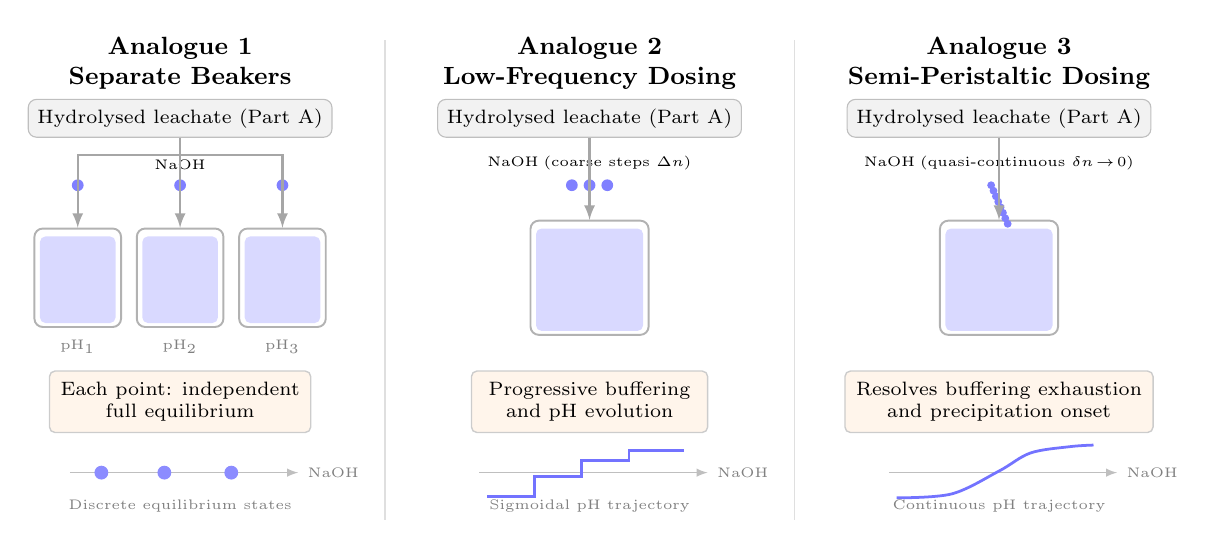
\begin{tikzpicture}[
    font=\small,
    beaker/.style={draw=gray!60, fill=blue!6, rounded corners=3pt,
                   minimum width=1.1cm, minimum height=1.4cm, line width=0.7pt},
    drop/.style={circle, fill=blue!50, inner sep=1.5pt},
    arrow/.style={-latex, thick, gray!70},
    titlestyle/.style={font=\bfseries\small, align=center},
    tagbox/.style={draw=gray!40, fill=white, rounded corners=2pt,
                   inner sep=4pt, font=\scriptsize, align=center,
                   line width=0.5pt, minimum width=3.0cm},
    tagboxO/.style={draw=gray!40, fill=orange!8, rounded corners=2pt,
                   inner sep=4pt, font=\scriptsize, align=center,
                   line width=0.5pt, minimum width=3.0cm},
]

% ── column x-centres ──
\def\xA{0}      % Analogue 1
\def\xB{5.2}    % Analogue 2
\def\xC{10.4}   % Analogue 3

% ── vertical anchors (increase gaps here to push items apart) ──
\def\yHeader{0.25}     % column titles
\def\ySrc{-0.45}       % leachate source box
\def\yDrop{-1.30}      % NaOH drops / label
\def\yBeaker{-2.50}    % beaker centres
\def\yPHlabel{-3.35}   % pH label below beakers
\def\yTag1{-4.10}      % first tag box
\def\yTag2{-4.05}      % second tag box
\def\ySketchAx{-4.95}  % pH sketch axis
\def\ySketchLb{-5.38}  % sketch label
\def\yBar{-5.20}       % bottom output bar
\def\yDivBot{-5.55}    % divider bottom

% ════════════════════════════════════════════════════════════════════
% HEADER ROW
% ════════════════════════════════════════════════════════════════════
\node[titlestyle] at (\xA, \yHeader)  {Analogue 1\\Separate Beakers};
\node[titlestyle] at (\xB, \yHeader)  {Analogue 2\\Low-Frequency Dosing};
\node[titlestyle] at (\xC, \yHeader)  {Analogue 3\\Semi-Peristaltic Dosing};

% ── column dividers ──
\draw[gray!25, line width=0.5pt] (2.6,\yDivBot) -- (2.6,0.55);
\draw[gray!25, line width=0.5pt] (7.8,\yDivBot) -- (7.8,0.55);

% ════════════════════════════════════════════════════════════════════
% ANALOGUE 1 — three independent beakers
% ════════════════════════════════════════════════════════════════════

\node[draw=gray!50, fill=gray!10, rounded corners=3pt,
      minimum width=3.4cm, minimum height=0.45cm, font=\scriptsize]
      (src1) at (\xA,\ySrc) {Hydrolysed leachate (Part A)};

% beakers
\foreach \i in {1,2,3}{
    \pgfmathsetmacro\bx{\xA - 1.3 + (\i-1)*1.3}
    % liquid
    \fill[blue!15, rounded corners=2pt]
        (\bx-0.48,\yBeaker-0.55) rectangle (\bx+0.48,\yBeaker+0.55);
    \draw[gray!60, line width=0.7pt, rounded corners=3pt]
        (\bx-0.55,\yBeaker-0.60) rectangle (\bx+0.55,\yBeaker+0.65);
    % drop
    \node[drop] at (\bx,\yDrop) {};
    % label below
    \node[font=\tiny, gray] at (\bx,\yPHlabel) {pH$_\i$};
}
\node[font=\tiny, above=2pt] at (\xA,\yDrop) {NaOH};

% arrows leachate → beakers
\draw[arrow] (src1.south) -- ++(0,-0.22) -| (\xA-1.3,\yBeaker+0.66);
\draw[arrow] (src1.south) -- ++(0,-0.22) -- (\xA,\yBeaker+0.66);
\draw[arrow] (src1.south) -- ++(0,-0.22) -| (\xA+1.3,\yBeaker+0.66);

% tag boxes
%\node[tagbox]  at (\xA,\yTag1) {No chemical memory\\between beakers};
\node[tagboxO] at (\xA,\yTag2) {Each point: independent\\full equilibrium};

% pH sketch
\draw[-latex, gray!50, thin]
    (\xA-1.4,\ySketchAx) -- (\xA+1.5,\ySketchAx)
    node[right, font=\tiny, gray] {NaOH};
\foreach \x in {-1.0,-0.2,0.65}{
    \fill[blue!45] (\xA+\x,\ySketchAx) circle (2.5pt);
}
\node[font=\tiny, gray] at (\xA,\ySketchLb) {Discrete equilibrium states};

% ════════════════════════════════════════════════════════════════════
% ANALOGUE 2 — single beaker, coarse steps
% ════════════════════════════════════════════════════════════════════

\node[draw=gray!50, fill=gray!10, rounded corners=3pt,
      minimum width=3.4cm, minimum height=0.45cm, font=\scriptsize]
      (src2) at (\xB,\ySrc) {Hydrolysed leachate (Part A)};

% beaker
\fill[blue!15, rounded corners=2pt]
    (\xB-0.68,\yBeaker-0.65) rectangle (\xB+0.68,\yBeaker+0.65);
\draw[gray!60, line width=0.7pt, rounded corners=3pt]
    (\xB-0.75,\yBeaker-0.70) rectangle (\xB+0.75,\yBeaker+0.75);

% coarse drops
\foreach \i in {1,2,3}{
    \node[drop] at (\xB-0.45+\i*0.225,\yDrop) {};
}
\node[font=\tiny, above=2pt] at (\xB,\yDrop) {NaOH\;(coarse steps $\Delta n$)};

\draw[arrow] (src2.south) -- (\xB,\yBeaker+0.76);

% tag boxes
%\node[tagbox]  at (\xB,\yTag1) {Chemical memory preserved\\across steps};
\node[tagboxO] at (\xB,\yTag2) {Progressive buffering\\and pH evolution};

% staircase sketch
\draw[-latex, gray!50, thin]
    (\xB-1.4,\ySketchAx) -- (\xB+1.5,\ySketchAx)
    node[right, font=\tiny, gray] {NaOH};
\draw[blue!55, line width=1pt]
    (\xB-1.3,\ySketchAx-0.30) -- (\xB-0.7,\ySketchAx-0.30) --
    (\xB-0.7,\ySketchAx-0.05) -- (\xB-0.1,\ySketchAx-0.05) --
    (\xB-0.1,\ySketchAx+0.15) -- (\xB+0.5,\ySketchAx+0.15) --
    (\xB+0.5,\ySketchAx+0.28) -- (\xB+1.2,\ySketchAx+0.28);
\node[font=\tiny, gray] at (\xB,\ySketchLb) {Sigmoidal pH trajectory};

% ════════════════════════════════════════════════════════════════════
% ANALOGUE 3 — quasi-continuous peristaltic
% ════════════════════════════════════════════════════════════════════

\node[draw=gray!50, fill=gray!10, rounded corners=3pt,
      minimum width=3.4cm, minimum height=0.45cm, font=\scriptsize]
      (src3) at (\xC,\ySrc) {Hydrolysed leachate (Part A)};

% beaker
\fill[blue!15, rounded corners=2pt]
    (\xC-0.68,\yBeaker-0.65) rectangle (\xC+0.68,\yBeaker+0.65);
\draw[gray!60, line width=0.7pt, rounded corners=3pt]
    (\xC-0.75,\yBeaker-0.70) rectangle (\xC+0.75,\yBeaker+0.75);

% fine drip
\foreach \i in {0,...,7}{
    \node[drop, inner sep=1pt]
        at (\xC-0.10+\i*0.03, \yDrop-\i*0.07) {};
}
\node[font=\tiny, above=2pt] at (\xC,\yDrop)
    {NaOH\;(quasi-continuous $\delta n\!\to\!0$)};

\draw[arrow] (src3.south) -- (\xC,\yBeaker+0.76);

% tag boxes
%\node[tagbox]  at (\xC,\yTag1) {Maximum path resolution\\(converged limit)};
\node[tagboxO] at (\xC,\yTag2) {Resolves buffering exhaustion\\and precipitation onset};

% smooth curve sketch
\draw[-latex, gray!50, thin]
    (\xC-1.4,\ySketchAx) -- (\xC+1.5,\ySketchAx)
    node[right, font=\tiny, gray] {NaOH};
\draw[blue!55, line width=1pt, smooth]
    plot[tension=0.55] coordinates {
        (\xC-1.3,\ySketchAx-0.32)
        (\xC-0.6,\ySketchAx-0.27)
        (\xC-0.0,\ySketchAx+0.02)
        (\xC+0.4,\ySketchAx+0.25)
        (\xC+0.9,\ySketchAx+0.33)
        (\xC+1.2,\ySketchAx+0.35)};
\node[font=\tiny, gray] at (\xC,\ySketchLb) {Continuous pH trajectory};

% ════════════════════════════════════════════════════════════════════
% BOTTOM: shared output bar
% ════════════════════════════════════════════════════════════════════


\end{tikzpicture}
\caption{\textbf{Three NaOH dosing analogues.} Analogue~1: independent batch equilibria with no chemical memory. Analogue~2: cumulative incremental dosing with coarse step size. Analogue~3: quasi-continuous semi-peristaltic addition ($\delta n\!\to\!0$), the physically converged limit. All share the same hydrolysed leachate initial condition (Part~A).}
\label{fig:analogue_schematic}
\end{figure*}

%%%%%%%%
%%%%%%%

\subsection{High-Throughput SDL Experimentation and ICP Analysis}\label{sec:sdl}

A HTE experimental platform (Telescope Innovations) was used to independently map metal dissolution and precipitation behavior as a function of leachate dilution and base loading. All experiments were conducted using a single NMC532 battery leachate composition, with leachate concentration varied by dilution across a systematic matrix of well-plate conditions. The platform integrated tip-based automated liquid handling to aliquot stock leachate solutions and dispense NaOH reagent into individual 1\,mL vials across a systematic dilution matrix, with liquid classes defined separately for the viscous leachate and the aqueous base to ensure dispensing accuracy. Standardized protocols with automated data acquisition and metadata logging ensured reproducibility and traceability across all experimental conditions.

Dissolved metal concentrations in the SDL-generated samples were quantified by inductively coupled plasma optical emission spectrometry (ICP-OES) as a function of incremental base addition. Samples were taken before and after adding prescribed volumes of base, filtered to remove suspended solids, and analyzed to determine solution-phase metal concentrations. Experiments were conducted in small-volume reactors (1\,mL vials) using fixed NaOH-to-leachate dosing ratios; results are reported as normalized doses (per unit leachate volume) to enable direct comparison with equilibrium calculations performed at the liter scale. Experimental data are interpreted as reflecting net, system-scale metal removal under practical conditions, whereas thermodynamic calculations represent the idealized, well-mixed equilibrium limit; the implications of this distinction for comparing modeled and measured metal activities are discussed in the context of Fig.~\ref{fig:free_ion}.



%%%%%
%%%%%

\section{Results and Discussion}\label{sec:results}

%\subsection{Simulation Scenario}

The following results are organized according to the two-stage framework and three dosing analogues described in Section~\ref{sec:methods}: Part A addresses dissolution and hydrolysis confirming all six metals dissolve fully under the acidic, sulfate-rich initial conditions across the entire ensemble, establishing a chemically consistent baseline for neutralization. Part B addresses the neutralization trajectories for each analogue, revealing how precipitation selectivity, onset pH, and co-precipitation risk evolved as a function of dosing pathway and leachate composition. Fig.~\ref{fig:leaching} summarizes the uncertainty propagation from leachate composition inputs through hydrolysis equilibria to metal recovery under the separate beakers analogue (Fig.~\ref{fig:analogue_schematic}): (a) shows the joint distribution of sampled metal concentrations and NaOH loadings, (b) the metal dissolution fractions as a function of resulting leaching pH across all compositions, and (c) the hydroxide precipitation recovery curves as a function of NaOH dose.

\subsection{Part A: Metal Sulfate Dissolution and Hydrolysis}

Part A characterizes the pre-neutralization leachate across five aspects: the leachate chemistry and speciation, the reference composition thermodynamic state, the dominant controls on ionic strength, the stoichiometric correlation structure among cathode metals, and the pH drivers governing acidification across the full compositional space.

% ---- ORIGINAL TEXT (preserved for reference) ----
% We first investigated a chemically realistic hydrolyzed leachate representative of hydromethalurgical battery recycling streams prior to base addition. Metal sulfates (Al, Fe, Cu, Co, Ni, Mn) were dissolved in deionized water at 25~$^\circ$C, where multivalent cations underwent hydrolysis and sulfate complexation. These reactions generated acidity, produced intrinsic buffering, and yielded a speciation landscape dominated by hydroxo- and sulfate-complexed species. Although the initiated model initialized near neutral pH, the system rapidly equilibrated to acidic conditions. To ensure realistic feed variability, metal inputs were sampled from representative lithium-ion battery chemistries (e.g., NMC111-NMC811, NCA, LCO), where Ni, Mn, and Co (and Al in NCA) followed stoichiometric ratios with stochastic variation. Additional independent contributions from Al, Fe, and Cu accounted for black mass and hardware sources. A representative baseline instance from this sampling space was tabulated in Table~\ref{tab:baseline_leachate}. The equilibrated solution was acidic (pH~=~4.19) with ionic strength (2.21~mol\,kg$^{-1}$), reflecting the concentrated metal sulfate loading of this NMC532 reference composition; all metals remained essentially fully dissolved (${\sim}$100\%), confirming undersaturation with respect to all hydroxide phases. The negligible charge imbalance ($-1.94\times10^{-12}$) confirmed numerical consistency. The pe of 6.35 indicated mildly oxidizing conditions; at this redox potential Fe$^{2+}$ is the thermodynamically favored iron species (the Fe$^{3+}$/Fe$^{2+}$ boundary lies near pe~$\approx$~13 at pH~4). Across the 12{,}001-sample ensemble, ionic strength was the dominant control on solution chemistry (Fig.~\ref{fig:leaching_corr}). The correlation matrix revealed strong stoichiometric couplings among the NMC cathode metals: Co--Mn (0.89) was the dominant pair, with Co--Ni and Ni--Mn both moderate (0.42). This structure directly reflected the NMC stoichiometric hierarchy: as cathode chemistry shifted from NMC111 to NMC811, Co and Mn were the co-declining minority metals (both falling from $\sim$1/3 to $\sim$1/10 of the transition-metal fraction), while Ni rose in the opposite direction. Co and Mn therefore co-varied strongly across the ensemble, whereas Ni was partially anti-correlated with both, yielding the observed weaker Co--Ni and Ni--Mn couplings. Free sulfate activity (SO$_4^{2-}$) was strongly coupled to ionic strength (0.76), confirming that sulfate was the dominant ionic strength driver in this leachate system; Co and Mn also showed strong positive correlations with free SO$_4^{2-}$ (0.74 each), consistent with their large sulfate inputs, while Fe showed near-zero correlation (0.03), reflecting near-complete sequestration of Fe-associated sulfate into the FeSO$_4$ complex. Among the pH correlations, Al loading exerted the strongest acidifying effect ($r = -0.82$), consistent with Al$^{3+}$ being one of the most strongly hydrolyzing cations: the reaction Al$^{3+}$ + 3H$_2$O $\rightleftharpoons$ Al(OH)$_3$(s) + 3H$^+$ releases three protons per mole, depressing the equilibrium pH significantly~\cite{stumm_aquatic_1996, may_gibbsite_1979}. Fe loading was the second strongest pH driver ($r = -0.64$), reflecting Fe$^{3+}$ hydrolysis, while Cu, Ni, Co, and Mn showed negligible pH correlations ($|r| \leq 0.14$), consistent with their weaker hydrolysis tendencies and independent LHS sampling. These couplings have practical implications for pH control: leachates with variable Al or Fe content exhibited systematic pH shifts that had to be accounted for in NaOH dosing strategies. All dissolution fractions remained near 100\% across the pre-neutralization pH range ($\approx$3.7--4.7) spanned by the LHS ensemble (Fig.~\ref{fig:leaching}(b)), confirming undersaturation with respect to all hydroxide phases prior to base addition.
% ---- END ORIGINAL TEXT ----

% P1 — Leachate chemistry and speciation
When metal sulfates (Al, Fe, Cu, Co, Ni, Mn) were dissolved and allowed to equilibrate at 25~$^\circ$C, the system acidified spontaneously from near-neutral initialization to strongly acidic conditions without any base addition. This acidification is thermodynamically driven: Al$^{3+}$ and Fe$^{3+}$ undergo hydrolysis releasing three protons per mole, while concurrent sulfate complexation partitioned dissolved metals between free ionic forms and neutral complexes (e.g., FeSO$_4$, CoSO$_4$, NiSO$_4$), reducing free-ion activities below total dissolved concentrations. This speciation shift has a direct consequence for phase stability: because $K_{sp}$ is defined in terms of free-ion activities rather than total dissolved concentrations, the effective solubility threshold for each hydroxide phase is reached at a higher total metal concentration than simple solubility product arguments would suggest.

% P2 — Reference composition thermodynamic state
The model suggests that the NMC532 reference leachate equilibrated to pH~=~4.19 with ionic strength 2.21~mol~kg$^{-1}$ (Table~\ref{tab:baseline_leachate}), far exceeding the validity range of extended Debye-H\"uckel formalisms (typically $\leq$0.5~mol~kg$^{-1}$) and confirming that SIT-level activity corrections were essential for this system. All six metals remained essentially fully dissolved (${\sim}$100\%), consistent with undersaturation with respect to all hydroxide phases. At pe~=~6.35, applying the Nernst equation gave $\log(a_{\mathrm{Fe^{3+}}}/a_{\mathrm{Fe^{2+}}}) = \mathrm{pe} - \mathrm{pe}^\circ = 6.35 - 13.03 = -6.68$, meaning Fe$^{3+}$ was suppressed by nearly seven orders of magnitude relative to Fe$^{2+}$. Dissolved iron therefore existed almost entirely as Fe$^{2+}$ in the pre-neutralization leachate, despite Fe(OH)$_3$(s) being the thermodynamically stable iron solid, a distinction with direct consequences for predicting the pH at which iron precipitation onset occurs. The negligible charge imbalance ($-1.94\times10^{-12}$~mol~kg$^{-1}$) confirmed the numerical consistency of the equilibrium solution.

% P3 — Ionic strength dominance
Ionic strength was the dominant control on solution chemistry across all compositions (Fig.~\ref{fig:leaching_corr}), reflecting the intrinsically high salt loading of concentrated battery leachates. This dominance has a clear physical basis: sulfate, the principal anion, carries $z = -2$ and contributes four times more to $I = \tfrac{1}{2}\sum z^2 m$ per mole than monovalent ions. The strong coupling between free SO$_4^{2-}$ activity and ionic strength ($r = 0.76$) confirmed sulfate as the principal ionic strength driver. Co and Mn showed strong positive correlations with free SO$_4^{2-}$ ($r = 0.74$ each), consistent with their large sulfate inputs, whereas Fe showed near-zero correlation ($r = 0.03$), reflecting near-complete sequestration of Fe-associated sulfate into the neutral FeSO$_4$ complex. This has an important implication for activity modeling: SIT corrections matter most for the highest-charge species (Al$^{3+}$, Fe$^{3+}$), making rigorous activity modeling most critical precisely for the impurity metals that precipitate first.

% P4 — Stoichiometric correlation structure
The correlation matrix revealed a clear stoichiometric coupling structure among the NMC cathode metals. Co and Mn were most strongly correlated ($r = 0.89$), while Co--Ni and Ni--Mn were moderate ($r = 0.42$). This pattern is a direct consequence of the NMC unit-sum constraint: as Ni content rises from NMC111 to NMC811, Co and Mn both decline together, making them jointly declining minority metals across the compositional space while Ni was partially anti-correlated with both. This correlation structure propagated through the thermodynamic model as a correlated input pair: leachates with higher Co loading systematically carried higher Mn loading, broadening the joint uncertainty in the Co--Mn precipitation window and tightening the constraint on the operating pH for selective Cu removal before cathode metals began to precipitate.

% P5 — pH drivers and dissolution confirmation
Al loading exerted the strongest acidifying effect on pre-neutralization pH ($r = -0.82$), followed by Fe ($r = -0.64$), while Cu, Ni, Co, and Mn showed negligible contributions ($|r| \leq 0.14$). This hierarchy reflects hydrolysis stoichiometry: Al$^{3+}$ and Fe$^{3+}$ each release three protons per mole upon hydrolysis, the maximum yield in this system, whereas the divalent cathode metals release only two protons per mole with substantially weaker hydrolysis constants~\cite{stumm_aquatic_1996, may_gibbsite_1979}. Consequently, the pre-neutralization pH and the total NaOH demand for the neutralization stage are governed almost entirely by impurity loading rather than by the target cathode metals, requiring NaOH dosing strategies to be calibrated against Al and Fe variability as the primary pH-setting variables. All dissolution fractions remained near 100\% across the full pre-neutralization pH range ($\approx$3.7--4.7, Fig.~\ref{fig:leaching}(b)), confirming that the precipitation selectivity observed in Part B is determined entirely by hydroxide phase thermodynamics, not by incomplete dissolution at the leaching stage.



%%%%%
%%%%%
%%%%%

% --- Fig 3: LHS workflow (a)(b)(c) ---
\begin{figure*}[!ht]
\centering
    \begin{tikzpicture}
        \node (img1) at (0,0) {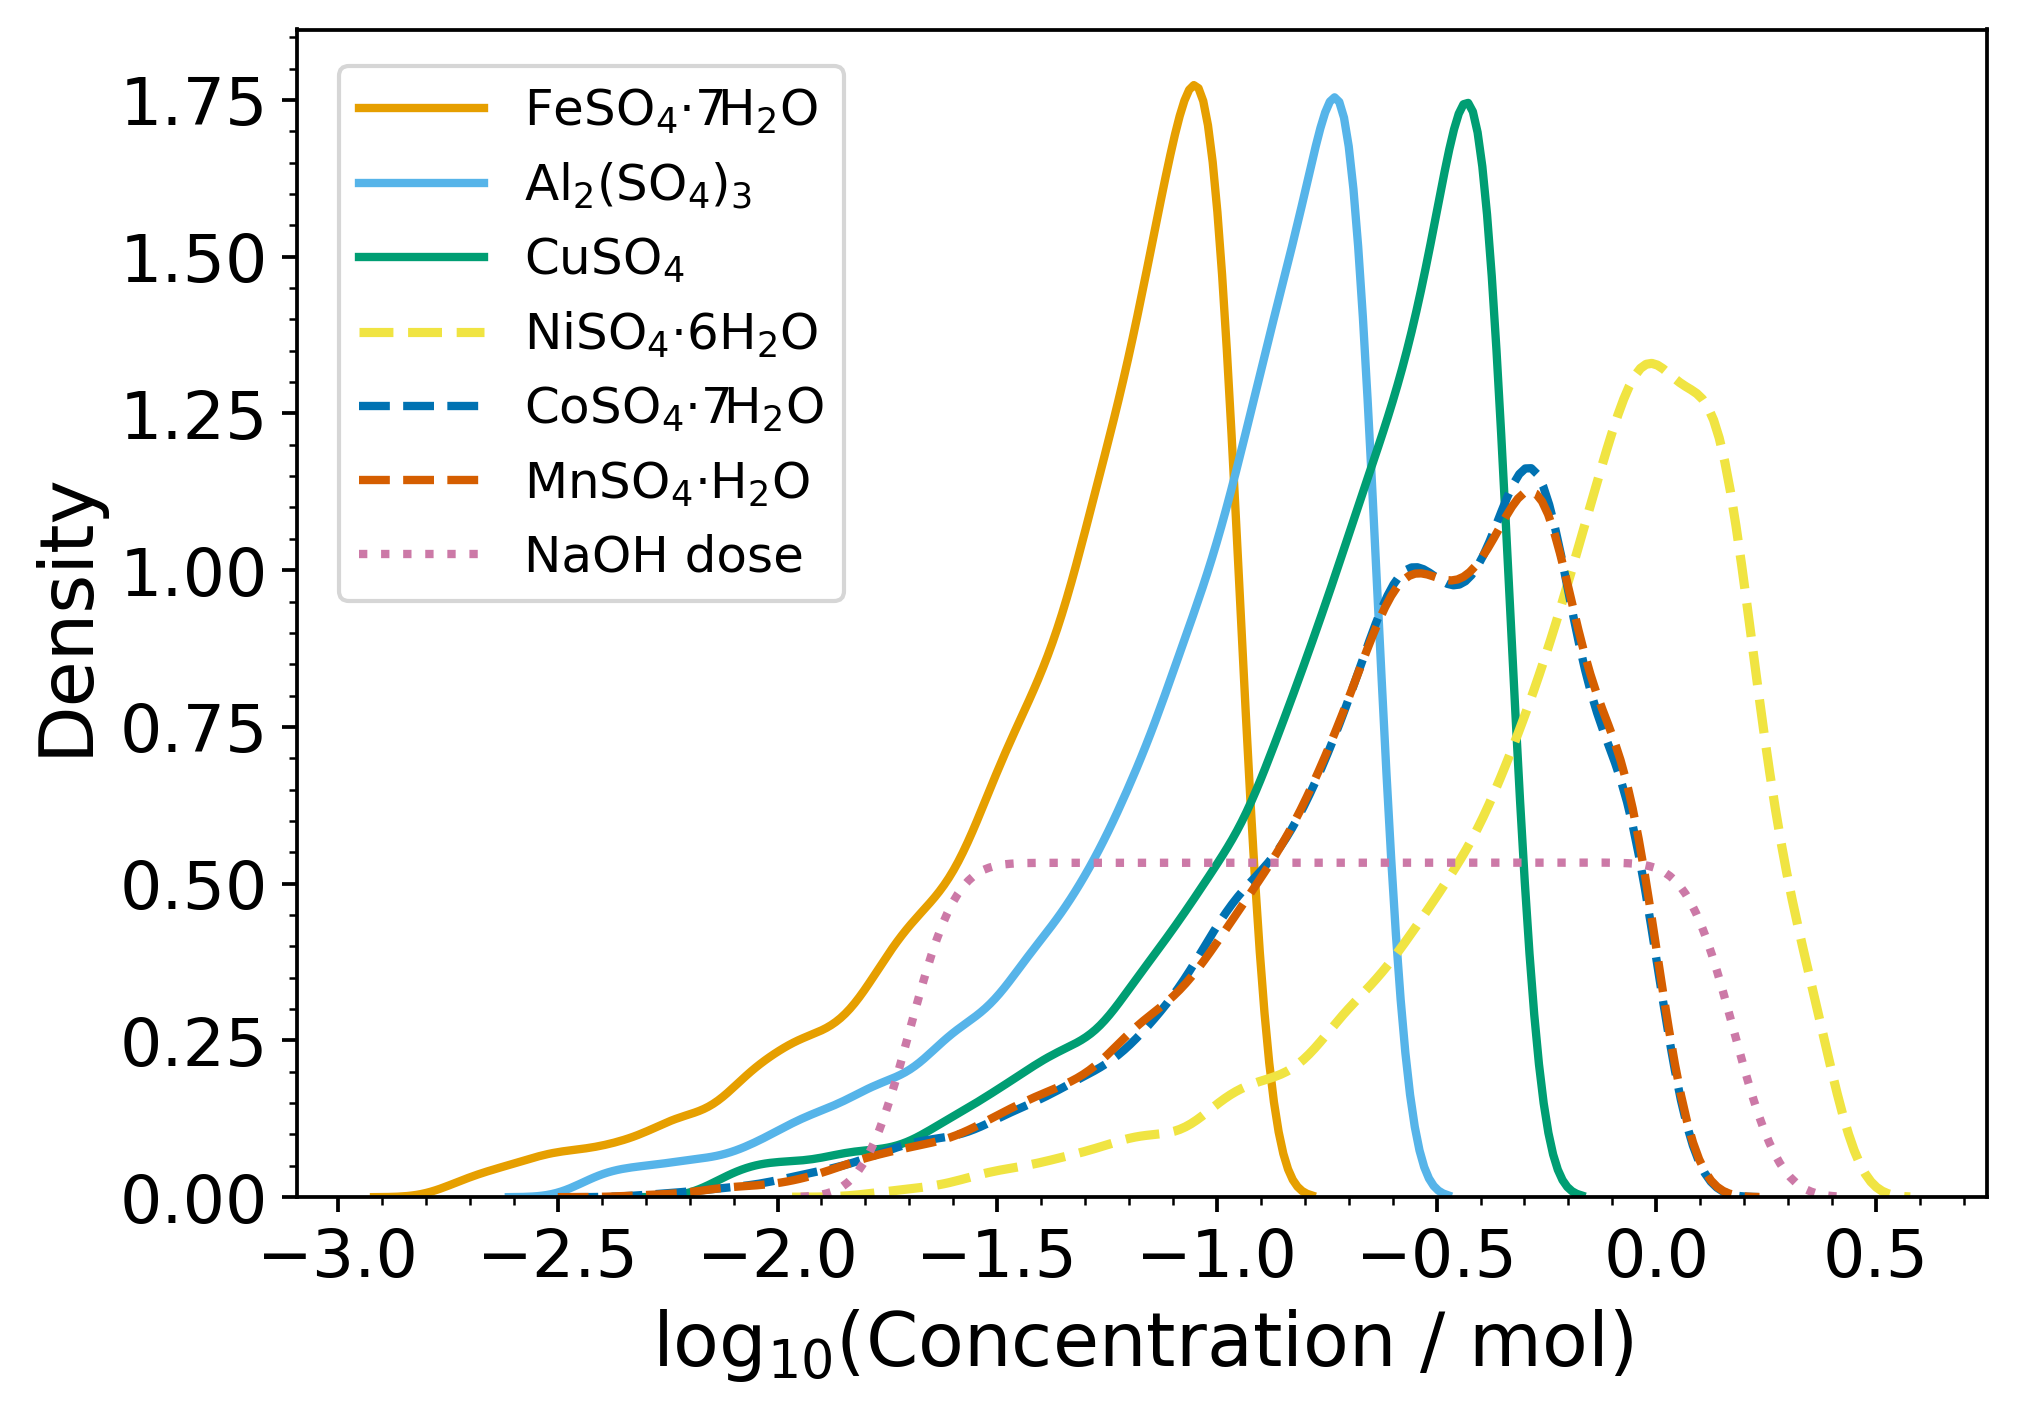
\includegraphics[width=0.34\linewidth]{results/Leach_recovery_UP6/fig_lhs_kde.png}};
        \node (img2) at (5.5,0) {\includegraphics[width=0.24\linewidth]{paper_SIT/Leach_recovery_UP6/figs_mix1/metal_dissolution_vs_pH.png}};
        \node (img3) at (11,0) {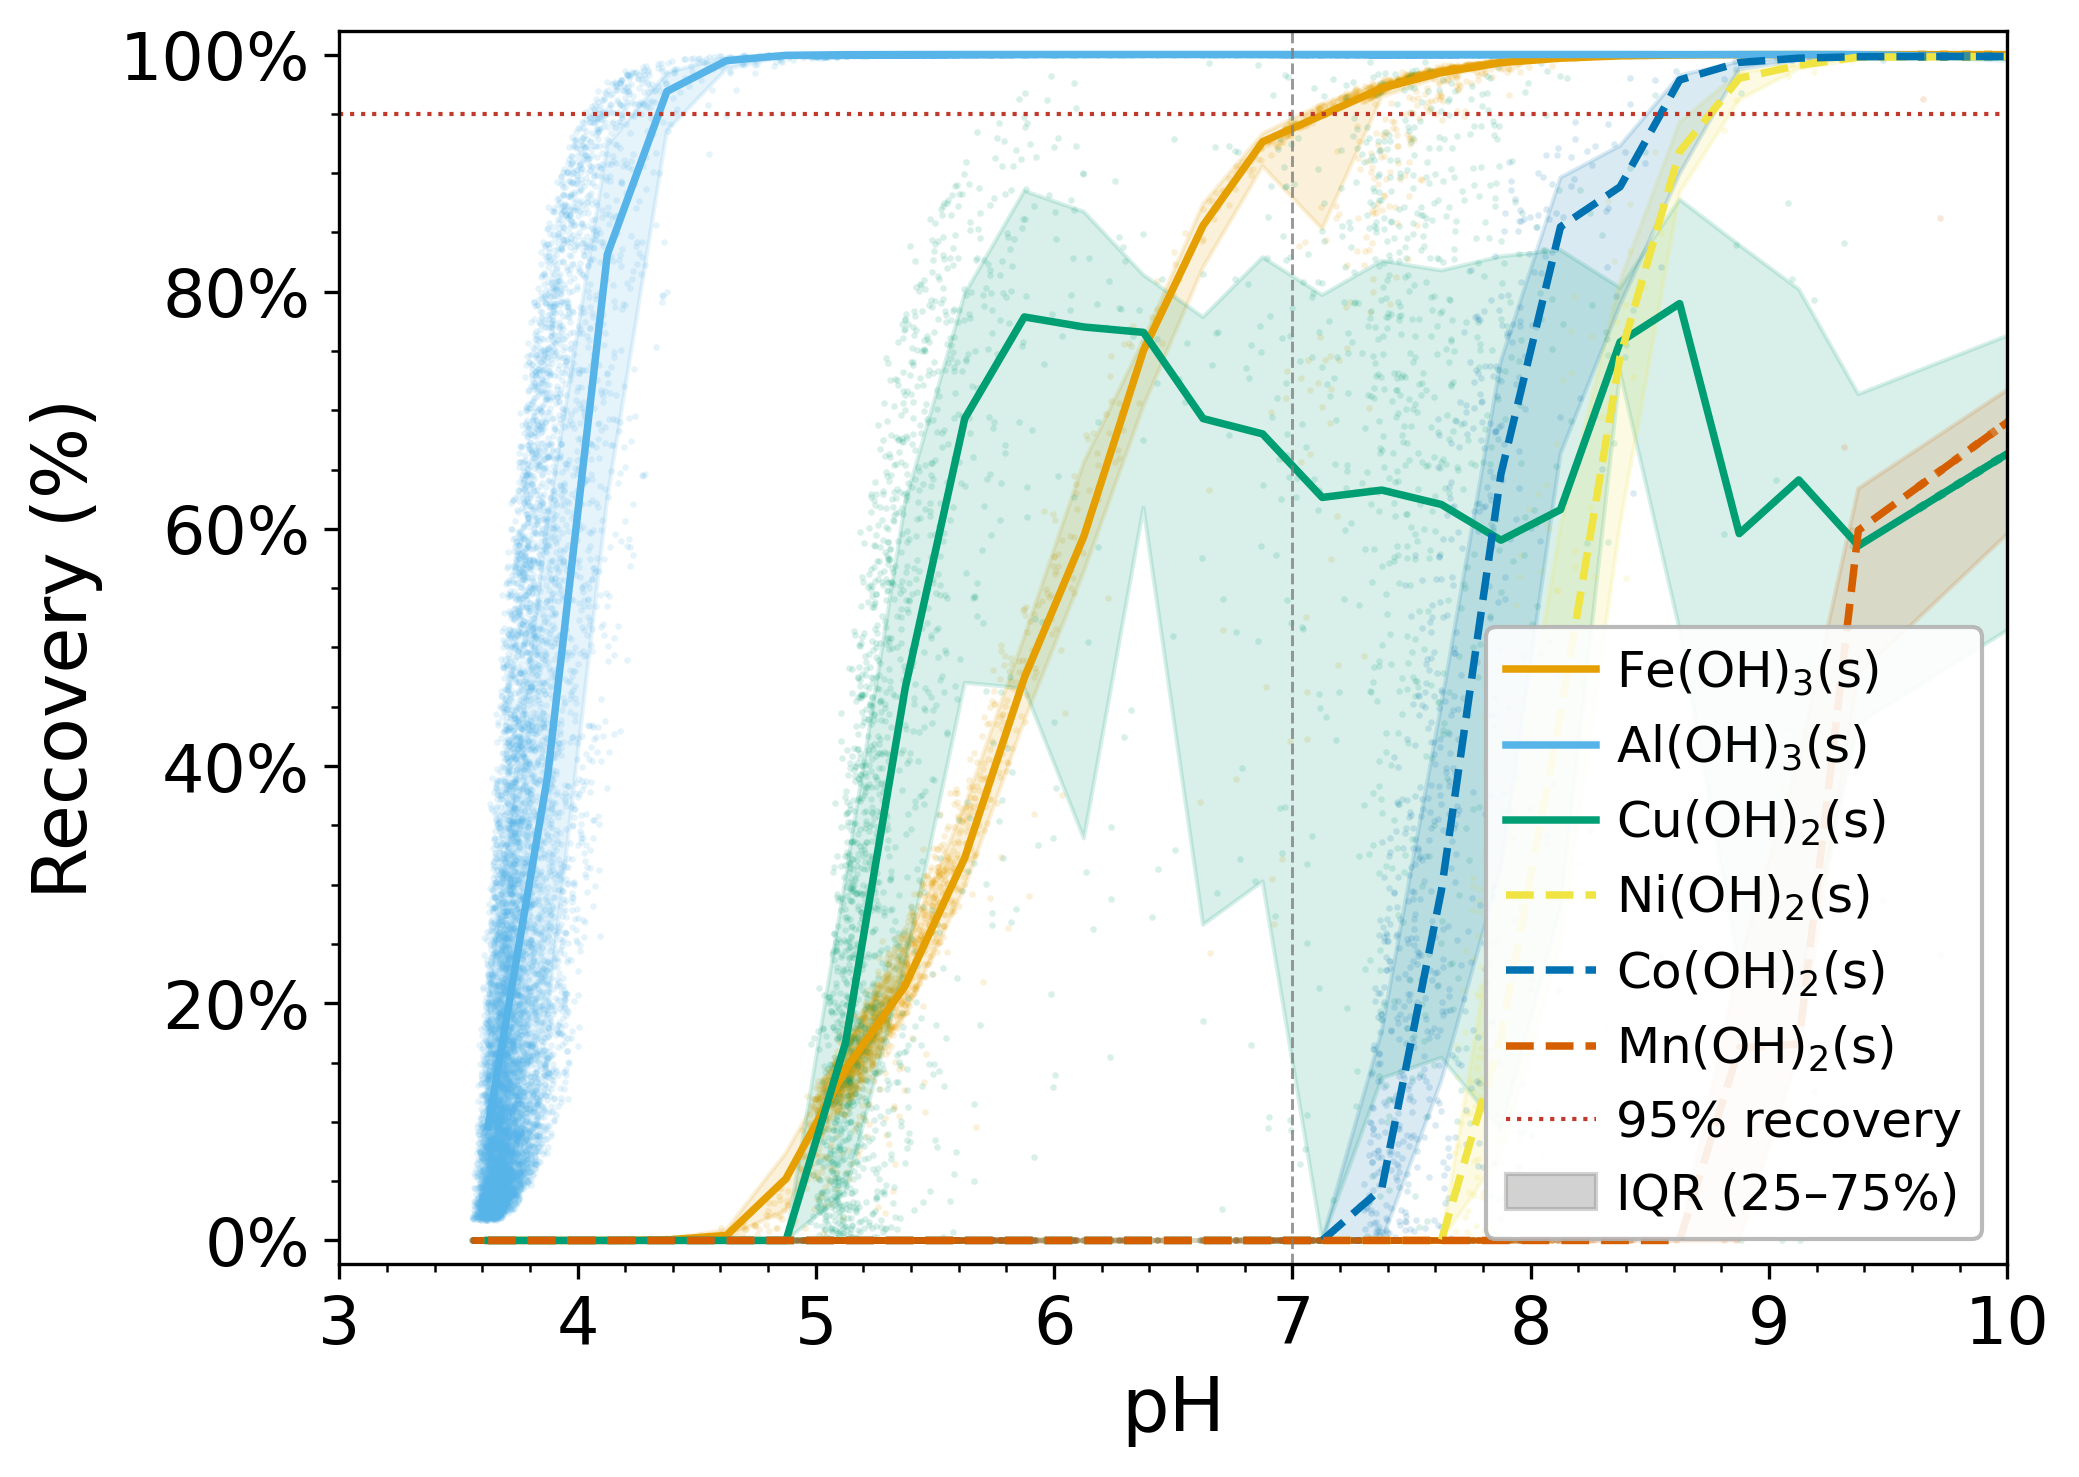
\includegraphics[width=0.34\linewidth]{results/Leach_recovery_UP6/figN2_recovery_direct_pct_eq.png}};
        \node[anchor=north west, font=\bfseries] at ($(img1.north west)+(-0.15,-0.1)$) {(a)};
        \node[anchor=north west, font=\bfseries] at ($(img2.north west)+(-0.15,-0.1)$) {(b)};
        \node[anchor=north west, font=\bfseries] at ($(img3.north west)+(-0.15,-0.1)$) {(c)};
        \draw[-latex, line width=2.2pt, gray!80]
            ($(img2.west)+(-0.5,0)$) -- ($(img1.east)+(0.6,0)$);
        \draw[-latex, line width=2.2pt, gray!80]
            ($(img3.west)+(-0.5,0)$) -- ($(img2.east)+(0.6,0)$);
    \end{tikzpicture}
\caption{
    \textbf{(a)} Joint distribution of sampled metal concentrations and NaOH loadings (log$_{10}$ scale).
    \textbf{(b)} Metal dissolution fraction versus pre-neutralization pH across all 12{,}001 compositions; near-complete dissolution ($\sim$100\%) confirms undersaturation with respect to all hydroxide phases prior to base addition.
    \textbf{(c)} Metal recovery versus NaOH dose (separate-beakers analogue).}
    \label{fig:leaching}
\end{figure*}

% --- Table: NMC532 reference leachate conditions ---
\begin{table}[!ht]
\centering
\caption{Computed equilibrium speciation of the NMC532 reference leachate at the pre-neutralization state (pH~4.19, $I = 2.21$~mol~kg$^{-1}$). All six metals are fully dissolved, establishing a chemically consistent baseline for the neutralization simulations.}
\label{tab:baseline_leachate}
\small
\setlength{\tabcolsep}{4pt}
\renewcommand{\arraystretch}{1.0}
\begin{tabularx}{0.60\linewidth}{p{2.8cm} p{2.5cm} cc}
\toprule
\textbf{Category} & \textbf{Variable} & \textbf{Value} & \textbf{Units} \\
\midrule
Operating conditions & Temperature & 25 & $^\circ$C \\
Process inputs & Leachate volume & 1.0 & L \\
\midrule
\multirow{6}{*}{Initial metal inventory}
 & Al$_2$(SO$_4$)$_3$      & 14.0  & g/L \\
 & Fe(SO$_4$)$_3$:7H$_2$O  & 5.6   & g/L \\
 & CuSO$_4$                 & 13.2  & g/L \\
 & CoSO$_4$:7H$_2$O         & 79.7  & g/L \\
 & NiSO$_4$:6H$_2$O         & 146.3 & g/L \\
 & MnSO$_4$:H$_2$O          & 41.9  & g/L \\
\midrule
\multirow{4}{*}{Bulk solution state}
 & pH               & 4.19                  & --              \\
 & pe               & 6.35                  & --              \\
 & Alkalinity       & $-9.53\times10^{-6}$  & eq\,L$^{-1}$   \\
 & Ionic strength   & 2.21                  & mol\,kg$^{-1}$ \\
\midrule
\multirow{6}{*}{Dissolved metals}
 & Al (total) & 0.074 & mol\,L$^{-1}$ \\
 & Fe (total) & 0.018 & mol\,L$^{-1}$ \\
 & Cu (total) & 0.075 & mol\,L$^{-1}$ \\
 & Co (total) & 0.257 & mol\,L$^{-1}$ \\
 & Ni (total) & 0.505 & mol\,L$^{-1}$ \\
 & Mn (total) & 0.225 & mol\,L$^{-1}$ \\
\midrule
\multirow{6}{*}{Dissolution fraction}
 & Al dissolved & $\sim$100 & \% \\
 & Fe dissolved & $\sim$100 & \% \\
 & Cu dissolved & $\sim$100 & \% \\
 & Co dissolved & $\sim$100 & \% \\
 & Ni dissolved & $\sim$100 & \% \\
 & Mn dissolved & $\sim$100 & \% \\
\midrule
Mass/charge closure & Charge imbalance & $-1.94\times10^{-12}$ & -- \\
\bottomrule
\end{tabularx}
\end{table}

% --- Fig 4: Correlation heatmap + ionic strength vs pH ---
\begin{figure*}[!ht]
\centering
    \begin{overpic}[width=0.49\textwidth]{paper_SIT/Leach_recovery_UP6/figs_mix1/fig7b_correlation_heatmap_upper.png}
        \put(18,15){\small\textbf{(a)}}
    \end{overpic}%
    \hfill
    \begin{overpic}[width=0.49\textwidth]{paper_SIT/Leach_recovery_UP6/figs_mix1/fig5_mu_vs_pH.png}
        \put(10,12){\small\textbf{(b)}}
    \end{overpic}
\caption{
    \textbf{(a)} Spearman correlation matrix across the 12{,}001-composition ensemble; ionic strength dominates solution chemistry; Co--Mn coupling ($r = 0.89$) reflects NMC stoichiometry; Al and Fe are the primary pH drivers ($r = -0.82$, $-0.64$).
    \textbf{(b)} Ionic strength versus pH across all compositions; star marks the experimental NMC532 reference.}
    \label{fig:leaching_corr}
\end{figure*}



%This hydrolysis stage is identical for all neutralization simulation analogues. Differences in the results therefore arise exclusively from how hydroxide is introduced in Part B, not from differences in initial solution chemistry. The hydrolyzed solutionsummreized in Table~\ref{tab:baseline_leachate} serves as a chemically consistent reference state for all subsequent simulations.

%%%%%%
%%%%%%
%%%%%%
\subsection{Part B: NaOH Neutralization and Hydroxide Precipitation}

Neutralization of the leachate is modeled by introducing NaOH as a stoichiometric source of hydroxide, with pH evolution, hydroxide consumption, and metal precipitation tracked explicitly. Although thermodynamic equilibrium is enforced at each calculation step, the connectivity between equilibrium states differs across the three analogues (Fig.~\ref{fig:analogue_schematic}), leading to fundamentally different representations of the neutralization pathway. The path dependence observed here is not a kinetic artifact: it reflects the fact that a sequence of equilibrium steps can access a different final state than a single large perturbation delivering the same total NaOH load. The connectivity between equilibrium states (which precipitated are present as seeds for further growth, how much buffering capacity has been consumed, and how much dissolved metal has already been removed) differs across the three analogues and determines the final chemical outcome.

In the \textbf{separate-beakers analogue}, each beaker represents an independent batch reactor to which a fixed amount of NaOH is introduced through an explicit stoichiometric reaction. Therefore, each calculation represents an isolated batch system, and the resulting equilibrium states are not chemically connected. Each system is equilibrated individually involving hydrolysis, complexation, and precipitation. This analogue identifies equilibrium precipitation thresholds as a function of total hydroxide added but does not represent progressive hydroxide addition or buffering-controlled pH evolution. A complementary representation is also considered aqueous speciation equilibrium while suppressing precipitation, thereby constraining the system to remained fully dissolved. Despite identical initial conditions obtained from part A and hydroxide addition, the suppression of precipitation holds the system in a metastable state above its global Gibbs free energy minimum, allowing supersaturation and elevated dissolved metal concentrations to persist. This approach approximates kinetically limited conditions where precipitation is inhibited, whereas enforcing phase equilibrium yields the fully equilibrated state. The difference between these treatments thus quantifies the extent to which precipitation controls system speciation and metal partitioning.

In the \textbf{slow dosing with low frequency dosing}, NaOH is introduced cumulatively in discrete increments, with the equilibrated speciation of each step passed directly as the initial condition for the next. Each equilibrated state serves as the starting point for the next addition, preserving chemical memory across steps. This analogue captures the gradual consumption of hydroxide by hydrolysis, complexation, and precipitation reactions and produces sigmoidal pH trajectories characteristic of controlled neutralization experiments. However, the finite step size limits resolution of closely spaced buffering and precipitation events. The \textbf{semi-peristaltic dosing analogue} refines the incremental approach by introducing hydroxide in small, frequent increments, reducing the step size by an order of magnitude relative to the low-frequency analogue. This produces a quasi-continuous neutralization trajectory that closely reproduces laboratory titration experiments. This analogue resolves buffering exhaustion, precipitation onset, and phase growth with high fidelity and is treated as the physically converged limit of the neutralization pathway. Unless otherwise noted, thermodynamic interpretations are drawn primarily from this formulation.





\begin{figure*}[!ht]
    \centering

    % ---- Row 1: SIT pathway (pH+pe inset | ionic strength+alkalinity inset) ----
    \begin{overpic}[width=0.48\textwidth]{paper_SIT/HH_results_initTrue_NaOH25_new/NaOH_vs_pH_all_experiments.png}%
        \put(-5,25){\rotatebox{90}{\small\textbf{Solution state}}}
        \put(2,68){\textbf{(a)}}
        \put(12,29){\includegraphics[width=0.21\textwidth]{paper_SIT/HH_results_initTrue_NaOH25_new/NaOH_vs_pe_all_experiments.png}}
        \put(55,54){\textbf{(b)}}
    \end{overpic}%
    \begin{overpic}[width=0.48\textwidth]{paper_SIT/HH_results_initTrue_NaOH25_new/NaOH_vs_mu_all_experiments.png}%
        \put(2,68){\textbf{(c)}}
        \put(13,23){\includegraphics[width=0.25\textwidth]{paper_SIT/HH_results_initTrue_NaOH25_new/NaOH_vs_Alk_all_experiments.png}}
        \put(65,54){\textbf{(d)}}
    \end{overpic}

    \vspace{1.5mm}

    % ---- Row 0: column headers ----
    \begin{minipage}[c]{0.33\linewidth}\centering\textbf{Separate Beakers}\end{minipage}
    \begin{minipage}[c]{0.33\linewidth}\centering\textbf{Low-Frequency Dosing}\end{minipage}
    \begin{minipage}[c]{0.33\linewidth}\centering\textbf{Semi-Peristaltic Dosing}\end{minipage}

    \vspace{2mm}

    % ---- Row 2: total dissolved metal ----
    \begin{overpic}[width=0.33\linewidth]{paper_SIT/HH_results_initTrue_NaOH25_new/NaOH_vs_TotalMetalConc_experiment_HH_test_reaction_incrementalFalse_initTrue_NaOH25_new.png}
        \put(-7,25){\rotatebox{90}{\small\textbf{Dissolved metals}}}
        \put(2,70){\textbf{(e)}}
    \end{overpic}%
    \begin{overpic}[width=0.33\linewidth]{paper_SIT/HH_results_initTrue_NaOH25_new/NaOH_vs_TotalMetalConc_experiment_HH_test_reaction_incrementalTrue_Freq20_initTrue_NaOH25_new.png}
        \put(2,70){\textbf{(f)}}
        \put(55,11){$\xrightarrow{\raisebox{0pt}{\text{\tiny{amphoteric}}}}$}
    \end{overpic}%
    \begin{overpic}[width=0.33\linewidth]{paper_SIT/HH_results_initTrue_NaOH25_new/NaOH_vs_TotalMetalConc_experiment_HH_test_reaction_incrementalTrue_Freq100_initTrue_NaOH25_new.png}
        \put(2,70){\textbf{(g)}}
        \put(40,28){$\xrightarrow{\raisebox{0pt}{\text{\tiny{amphoteric}}}}$}
    \end{overpic}

    \vspace{1mm}

    % ---- Row 3: solid phase formation ----
    \begin{overpic}[width=0.33\linewidth]{paper_SIT/HH_results_initTrue_NaOH25_new/NaOH_vs_PhaseConc_experiment_HH_test_reaction_incrementalFalse_initTrue_NaOH25_new.png}
        \put(-7,25){\rotatebox{90}{\small\textbf{Solid phases}}}
        \put(2,70){\textbf{(h)}}
    \end{overpic}%
    \begin{overpic}[width=0.33\linewidth]{paper_SIT/HH_results_initTrue_NaOH25_new/NaOH_vs_PhaseConc_experiment_HH_test_reaction_incrementalTrue_Freq20_initTrue_NaOH25_new.png}
        \put(2,70){\textbf{(i)}}
    \end{overpic}%
    \begin{overpic}[width=0.33\linewidth]{paper_SIT/HH_results_initTrue_NaOH25_new/NaOH_vs_PhaseConc_experiment_HH_test_reaction_incrementalTrue_Freq100_initTrue_NaOH25_new.png}
        \put(2,70){\textbf{(j)}}
    \end{overpic}

    \caption{\textbf{Path-dependent neutralization response across three NaOH dosing analogues (SIT activity model).}
    \textbf{(a)} pH and \textbf{(b)} redox potential (pe, inset), \textbf{(c)} ionic strength and \textbf{(d)} alkalinity (inset) as a function of cumulative NaOH addition; despite identical NaOH loading, dosing pathway governs the chemical trajectory.
    \textbf{(e--g)} Total dissolved metal concentration and \textbf{(h--j)} solid phase formation for separate-beaker, low-frequency, and semi-peristaltic analogues, respectively. Amphoteric re-dissolution of Al, Cu, Co, and Mn is visible under incremental dosing (f,g). Differences in precipitation onset and phase accumulation directly reflect pathway-dependent buffering and hydroxide carryover.}
    \label{fig:neutralization_pathways}
\end{figure*}

Figure~\ref{fig:neutralization_pathways} presents the path-dependent evolution of solution chemistry and metal partitioning during NaOH neutralization of a hydrolyzed leachate under the three dosing analogues. Fig.~\ref{fig:neutralization_pathways}(a)--(d) capture bulk solution state; Fig.~\ref{fig:neutralization_pathways}(e)--(j) resolve metal-level dissolved and solid inventories across all three analogues.

% (a–d) Solution state
The pH response (Fig.~\ref{fig:neutralization_pathways}(a)) exhibit strong sensitivity to dosing mode. The separate-beaker analogue displays the most strongly buffered behavior, with delayed pH inflection reflecting complete equilibration at each NaOH addition. Low-frequency dosing shifted the trajectory to higher pH at comparable NaOH input, while semi-peristaltic dosing produces the earliest and steepest rise, signaling rapid exhaustion of buffering capacity. Redox potential (Fig.~\ref{fig:neutralization_pathways}(b)) closely paralleled pH: high-frequency dosing induced an abrupt pe collapse at substantially lower NaOH than the batch case, accelerating access to precipitation-relevant alkaline regimes. Ionic strength (Fig.~\ref{fig:neutralization_pathways}(c)) accumulated rapidly under semi-peristaltic dosing, reflecting retention of dissolved species during rapid additions, whereas the separate-beaker analogue maintained the lowest ionic strength throughout. Alkalinity (Fig.~\ref{fig:neutralization_pathways}(d)) provided a direct measure of hydroxide carryover: negligible under batch equilibration, stepwise under low-frequency dosing, and substantial under high-frequency addition where hydroxide injection outpaced hydrolysis and precipitation.

% (e–g) Total dissolved metal concentrations
In the separate-beaker analogue (Fig.~\ref{fig:neutralization_pathways}(e)), dissolved metal concentrations decreased in a stepwise, metal-specific sequence with increasing NaOH, consistent with equilibrium precipitation thresholds. Al was removed first, followed by Fe, then Cu, while Co, Ni, and Mn persisted to higher NaOH additions. Under incremental dosing (Fig.~\ref{fig:neutralization_pathways}(f) and (g)), several metals exhibited pronounced concentration minima followed by re-dissolution at high NaOH, most notably Al, Cu, Mn, and Co, a direct signature of amphoteric hydroxide chemistry. Ni showed negligible re-dissolution, consistent with its weak amphoteric character.

% (h–j) Solid phase formation
Solid phase formation mirrored the dissolved-phase trends. In the separate-beaker analogue (Fig.~\ref{fig:neutralization_pathways}(h)), each hydroxide phase appeared at a distinct NaOH threshold and grew monotonically, reflecting the thermodynamic precipitation sequence. Under incremental dosing (Fig.~\ref{fig:neutralization_pathways}(i) and (j)), phase onset was distributed over broader NaOH ranges and some phases subsequently declined at high pH due to amphoteric re-dissolution of previously formed solids, confirming that pH alone does not uniquely determine sustained solid formation under sequential dosing conditions.

%%%%%%%%%
%%%%%%%%%
%%%%%%%%%

\subsection{Thermodynamic Driving Forces: Saturation Index Evolution}

Figure~\ref{fig:precipitation_landscape} consolidates two thermodynamically complementary views of the precipitation landscape extracted from separate beakers calculations: the saturation index evolution (Fig.~\ref{fig:precipitation_landscape}(a)) and the phase-equilibrium onset pH distributions with selectivity windows (Fig.~\ref{fig:precipitation_landscape}(b)). For the remainder of this article, we focus only on separate beakers analogy due to its relevance to our lab scale and SDL development.

Figure~\ref{fig:precipitation_landscape}(a) shows that under phase-equilibrium conditions the SI of every stable phase is pinned at or below zero throughout the neutralization trajectory, confirming that the equilibrium solver correctly enforces the solubility constraint: once $Q_p$ reached $K_{sp}^p$, the solver redistributes dissolved species to maintain SI~$\leq$~0. Phases not yet stable remained at strongly negative SI, confirming undersaturation. The SI inset, computed with precipitation suppressed, revealed the thermodynamic driving force available to overcome nucleation barriers~\cite{stumm_aquatic_1996, bard_electrochemical_2022}: Al(OH)$_3$(s) and Fe(OH)$_3$(s) accumulate SI exceeding 10$^1$--10$^2$ log units above saturation well before pH~7, reflecting their exceptionally low $K_{sp}$ values and confirming that nucleation of these phases is thermodynamically robust across the entire compositional ensemble. By contrast, Mn(OH)$_2$(s) crossed SI~=~0 only above pH~$\approx$~8.5--9 for the reference NMC532 composition and accumulated only modest supersaturation thereafter (SI~$<$~1), leaving a smaller thermodynamic driving force for precipitation relative to Al, Fe, and Cu.


\begin{figure*}[!h]
\centering
\newlength{\figAfiveheight}
\setlength{\figAfiveheight}{0.3336\linewidth}%
\begin{minipage}[t]{0.43\linewidth}
  \vspace{0pt}
  \begin{overpic}[width=\linewidth]{results/Leach_recovery_UP6/fig_SI_vs_pH_combined.png}
    \put(2,77){\textbf{(a)}}
  \end{overpic}
\end{minipage}
\hfill
\begin{minipage}[t]{0.5228\linewidth}
  \vspace{0pt}
  \begin{overpic}[height=\figAfiveheight]{results/Leach_recovery_UP6/fig10_combined_onset_selectivity_eq.png}
    \put(2,65){\textbf{(b)}}
  \end{overpic}
\end{minipage}
\caption{\textbf{Thermodynamic precipitation landscape under phase-equilibrium conditions across 12{,}001 LHS samples.}
\textbf{(a)} Saturation index (SI) of each solid hydroxide phase as a function of pH (SIT activity model). Main figure: phase-equilibrium enforced: SI is pinned at zero once a phase became stable. Inset: precipitation suppressed: SI rose freely above zero, revealing accumulated supersaturation under kinetically inhibited conditions. The dashed line marks SI~=~0.
\textbf{(b)} Precipitation onset pH distribution (phase-equilibrium, SI threshold $\geq -0.05$), with phases ordered by median onset pH. Boxes spanned Q1--Q3; vertical tick marks the median; whiskers extend to the data range; circles are outliers. Annotated $\Delta$pH values indicate the gap between consecutive median onsets, quantifying the selectivity window available between adjacent precipitation steps. (Best viewed in color; refer to the online version for interpretation.)}
\label{fig:precipitation_landscape}
\end{figure*}

Figure~\ref{fig:precipitation_landscape}(b) shows the precipitation onset pH distribution across 12{,}001 leachate compositions under the phase-equilibrium constraint (SI threshold $\geq -0.05$). The onset sequence Al(OH)$_3$(s) $\to$ Fe(OH)$_3$(s) $\to$ Cu(OH)$_2$(s) $\to$ Co(OH)$_2$(s) $\approx$ Ni(OH)$_2$(s) $\to$ Mn(OH)$_2$(s) was conserved across all compositions, establishing that the thermodynamic hierarchy reflects the relative solubility products of these phases within the concentration ranges characteristic of battery leachates, rather than being a composition-specific accident~\cite{stumm_aquatic_1996, noauthor_ksp_nodate, bard_electrochemical_2022}. Al(OH)$_3$(s) precipitated first with a median onset near pH~4, consistent with the exceptionally low $K_{sp}$ of gibbsite and the strong hydrolyzing tendency of Al$^{3+}$~\cite{may_gibbsite_1979, stumm_aquatic_1996}. Fe(OH)$_3$(s) followed, separated from Al(OH)$_3$(s) by $\Delta$pH~=~1.5, a window wide enough to support selective Al removal before Fe precipitation onset. Fe(OH)$_3$(s) and Cu(OH)$_2$(s) had essentially identical median onsets ($\Delta$pH~=~0.1), making their fractionation by pH control alone practically impossible; both precipitated as a coupled impurity burden that must be managed jointly~\cite{virolainen_removal_2017, zanoletti_review_2024}. The largest actionable gap in the sequence was Cu(OH)$_2$(s)$\to$Co(OH)$_2$(s) ($\Delta$pH~=~2.2), defining a robust window for selective removal of the impurity metals (Al, Fe, Cu) before the valuable cathode metals began to precipitate~\cite{zanoletti_review_2024, larouche_progress_2020}. Co(OH)$_2$(s) and Ni(OH)$_2$(s) co-precipitated within $\Delta$pH~=~0.3 of each other, forming a tightly coupled pair that cannot be resolved by pH control alone~\cite{swain_separation_2015, swain_separation_2016, rabah_recovery_2008}. Mn(OH)$_2$(s) was the last phase to precipitate, with a median onset at pH~$\approx$~12.6 ($\Delta$pH~=~4.7 from Ni(OH)$_2$(s)), confirming that quantitative Mn removal requires strongly alkaline conditions beyond the operating range relevant to Co and Ni recovery~\cite{noauthor_ksp_nodate, bard_electrochemical_2022, free_hydrometallurgy_2021}. Together, Fig.~\ref{fig:precipitation_landscape}(a) and (b) provide a quantitative, composition-resolved map of the achievable selectivity windows, defining the NaOH dose targets and selectivity windows required for model-guided selective metal recovery.

%%%%%%
%%%%%%
%%%%%%

\subsection{Speciation, Co-precipitation Risk, and Analytical Detectability}\label{sec:speciation_coprec}

Saturation index and onset pH alone describe \emph{when} each phase crossed its thermodynamic threshold, but they do not resolve the chemical identity of the dissolved metal fraction, the statistical likelihood that target metals co-precipitated with early-forming impurity phases, or how quickly free-ion activities fall below the analytical detection limit during neutralization. Figures~\ref{fig:speciation_panel}--\ref{fig:free_ion} integrate three complementary perspectives, namely aqueous speciation, dissolved-fraction removal curves, and free-ion activity suppression, into a self-consistent thermodynamic picture of the neutralization landscape, propagated through the leaching--precipitation model chain across the full compositional variability of battery leachates.

\begin{figure*}[!h]
  \centering
  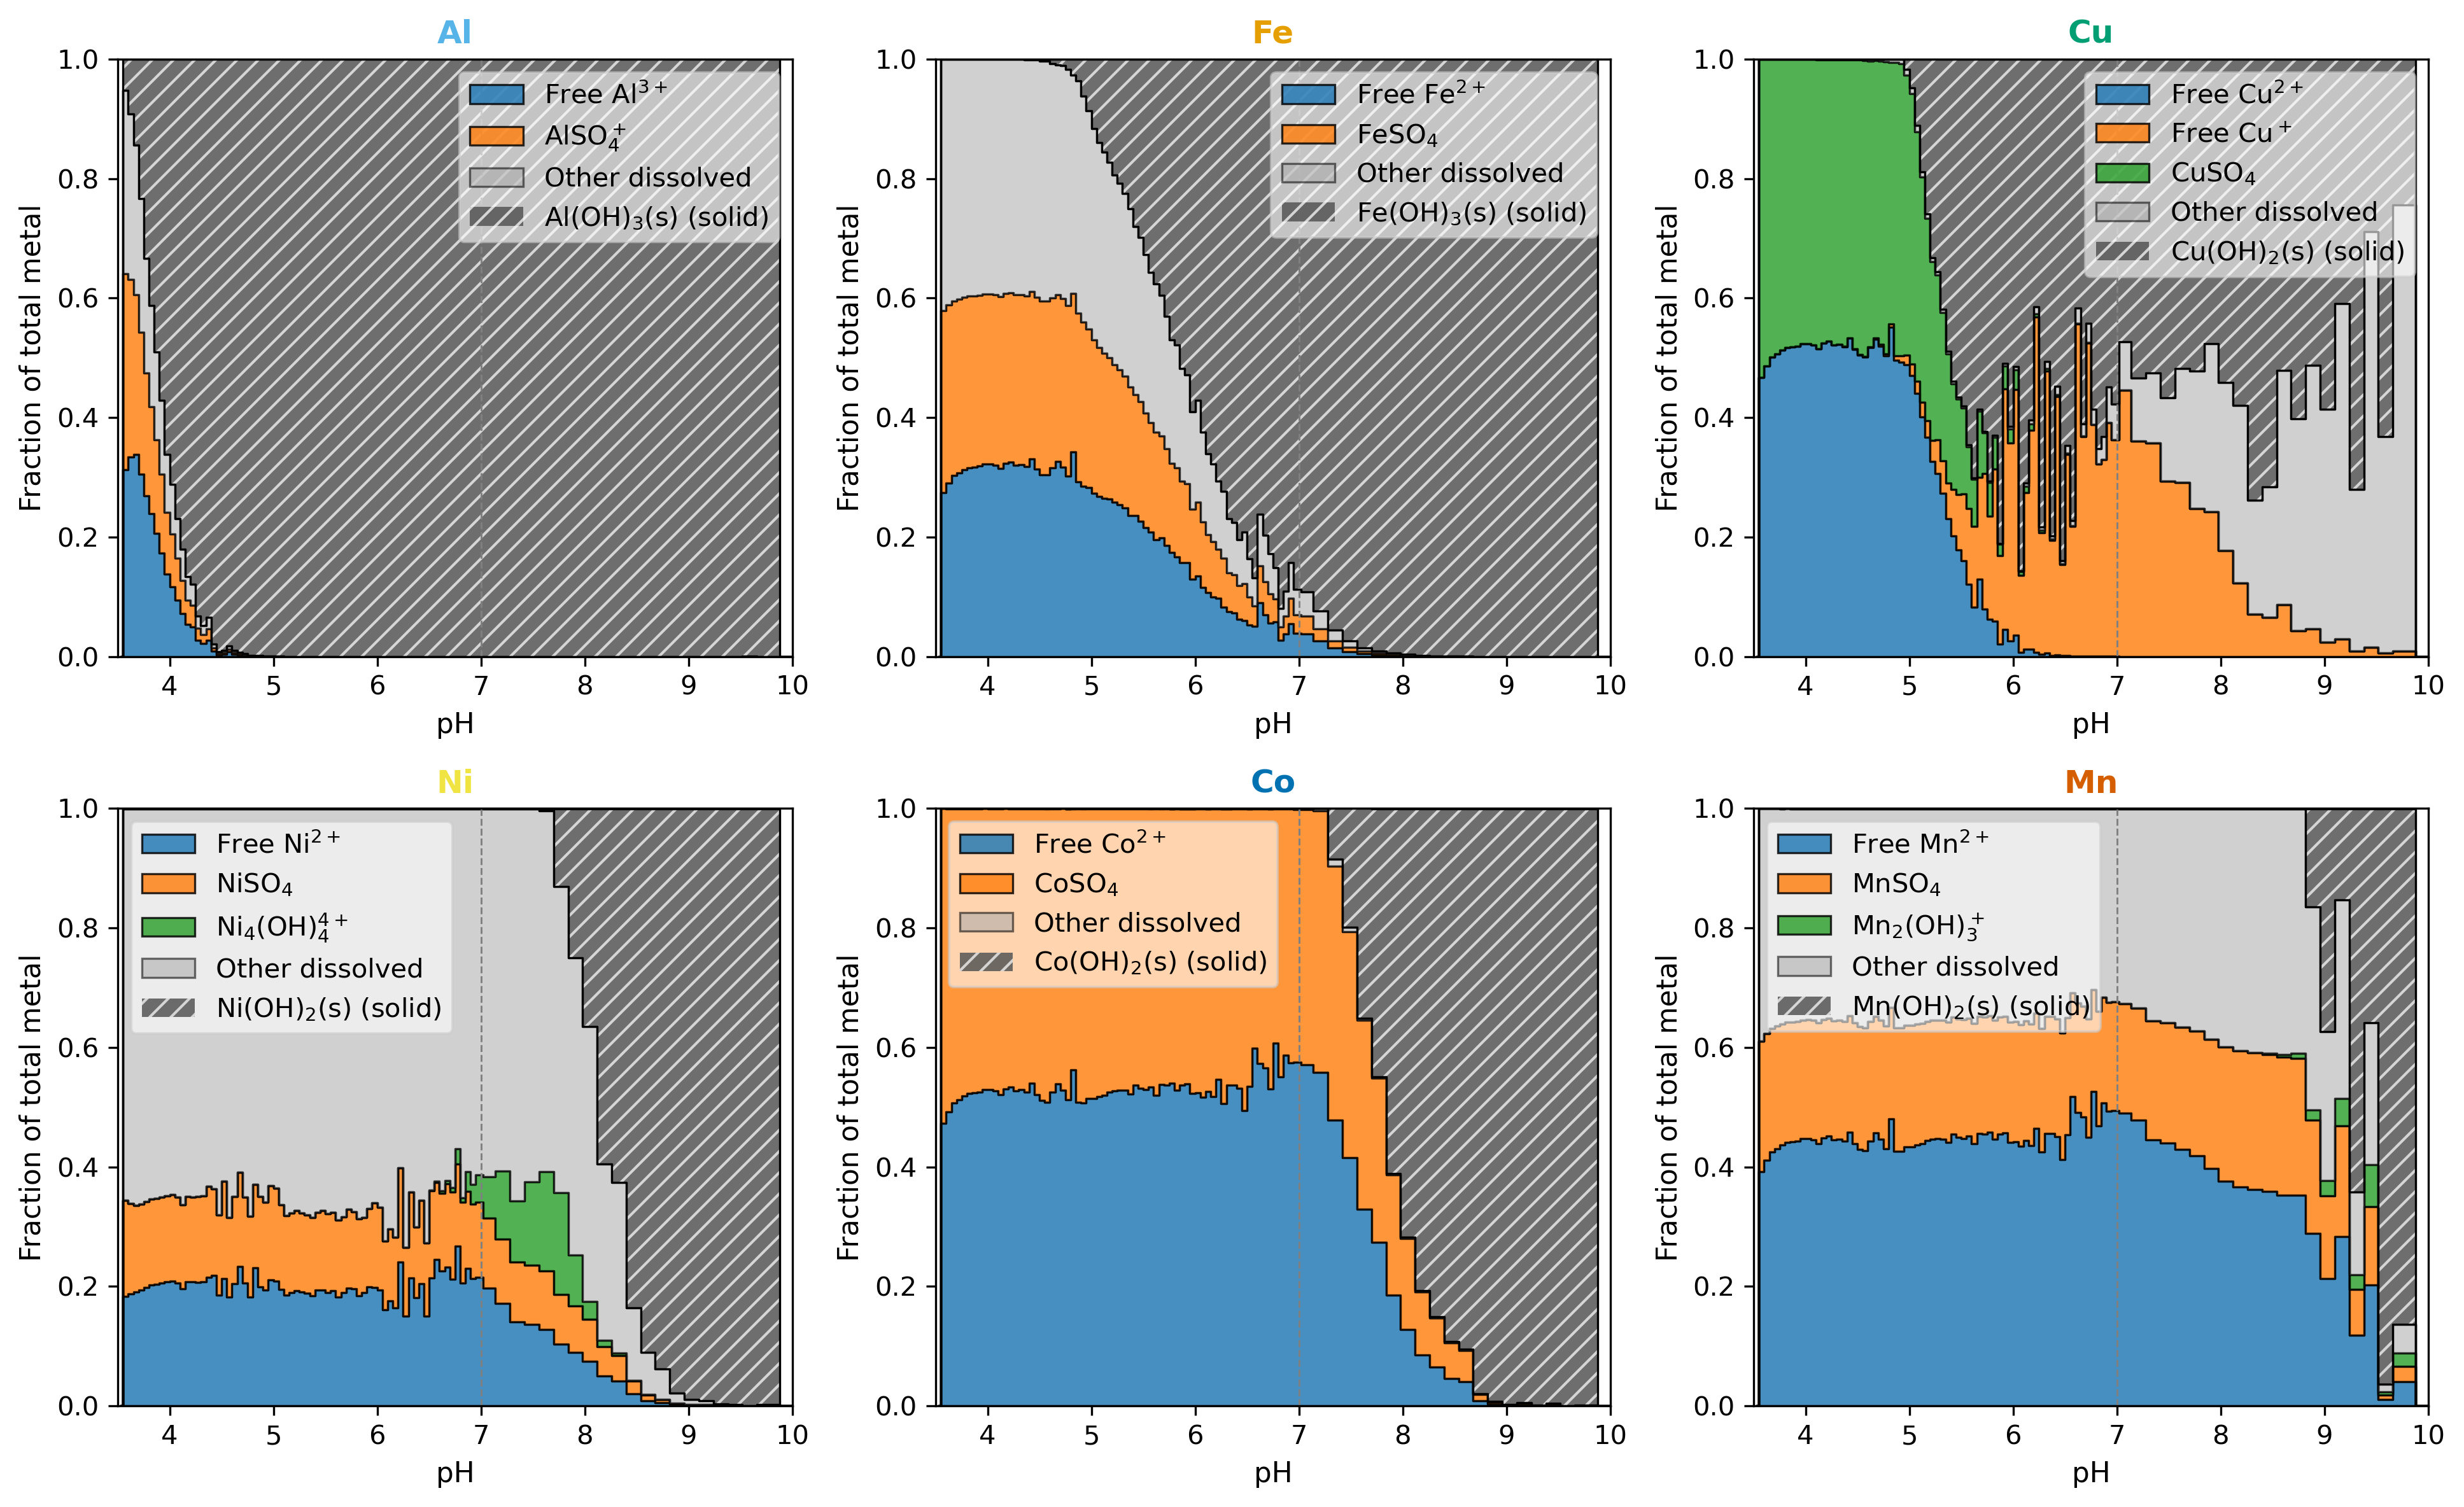
\includegraphics[width=\linewidth]{results/Leach_recovery_UP6/figC_speciation_with_solid_eq.png}
  \caption{\textbf{Total metal partitioning during NaOH neutralization.}
  Stacked area plots show the pH-dependent fraction of each metal in identified aqueous species, the solid hydroxide phase (white, black-hatched), and an unresolved dissolved fraction (``Other dissolved'', light gray), averaged across 12{,}001 leachate compositions (phase-equilibrium constraint; SIT activity model). Stacked areas sum to unity at each pH. The vertical dashed line marks pH~7. FeSO$_4$ is the neutral Fe$^{2+}$ sulfate complex; FeSO$_4^+$ is the Fe$^{3+}$ analogue. The ``Other dissolved'' fraction reflects SIT-implicit ion-pairing not captured by any individually resolved species (see text).}
  \label{fig:speciation_panel}
\end{figure*}

% Dissolution speciation controls precipitation precursors.
Unlike a Pourbaix diagram, which maps thermodynamic stability fields at a fixed metal activity and does not resolve speciation fractions, concentration effects, or multicomponent interactions, the speciation maps in Fig.~\ref{fig:speciation_panel} quantify how the total metal budget was distributed across aqueous species and the solid phase as a function of pH, averaged over the full compositional variability of realistic battery leachates under SIT-corrected activity modeling. The dominant dissolved form of each metal evolved with pH and governed the approach to precipitation. Al was dominated by free Al$^{3+}$ across the pre-precipitation pH range, transitioning to Al(OH)$_2^+$ as pH rose toward and above the Al(OH)$_3$(s) onset. For Fe, free Fe$^{2+}$ was the dominant explicitly-resolved species at low pH, consistent with the mildly oxidizing pe~=~6.35 of the leachate; Fe$^{3+}$ and its hydroxo complexes were negligible under these redox conditions. The solid Fe(OH)$_3$(s) band grew rapidly above pH~5, consuming essentially all dissolved Fe by pH~7.

The precipitation onset of Cu(OH)$_2$(s) was shifted to higher pH than a free-ion model would predict, a direct consequence of sulfate complexation sequestering nearly half of dissolved Cu as CuSO$_4$. Across pH~2--6, CuSO$_4$ accounted for $\sim$48\% of dissolved Cu, substantially reducing the free Cu$^{2+}$ activity below total dissolved Cu and delaying the crossing of the Cu(OH)$_2$(s) solubility threshold. An analogous effect governed Co speciation: CoSO$_4$ accounted for $\sim$48\% of dissolved Co at low pH, similarly suppressing the free Co$^{2+}$ activity relative to total dissolved Co. Because ICP-OES reports total dissolved metal without distinguishing free ions from sulfate complexes (Section~\ref{sec:sdl}), these sulfate-complexed fractions were analytically indistinguishable from free Cu$^{2+}$ and Co$^{2+}$, constituting an inherent offset between activity-corrected thermodynamic predictions and total-concentration ICP-OES measurements.

For Ni and Mn, a mechanistically distinct and substantially larger unresolved dissolved fraction was observed relative to the explicitly resolved sulfate complexes of Cu and Co. In Fig.~\ref{fig:speciation_panel}, the ``Other dissolved'' band represents metal accounted for in the total dissolved concentration (which sums \emph{all} dissolved forms) but not corresponding to any explicitly resolved aqueous species in the model output. At pH~$\approx$~4, this unresolved fraction accounted for $\sim$67\% of dissolved Ni and $\sim$36\% of dissolved Mn. For Ni and Mn, the origin of this gap is a fundamental feature of the SIT activity model: rather than defining ion pairs such as NiSO$_4$ or MnSO$_4$ as discrete aqueous species with explicit formation constants, the SIT formalism absorbs their thermodynamic effect into the activity coefficient of the free divalent cation through pairwise interaction parameters $\varepsilon(M^{2+}, \mathrm{SO_4^{2-}})$~\cite{guggenheim_specific_1955, noauthor_estimation_nodate}. For Al, the unresolved fraction likely reflects higher-order hydroxo-sulfate complexes and polymeric species not explicitly output by the model, rather than purely implicit SIT treatment. The calculated total dissolved metal correctly includes the full metal budget regardless of whether the association is treated as an explicit complex or an implicit SIT correction; the ``Other dissolved'' fraction is therefore not a model artifact or a data gap, but rather the combined thermodynamic signature of ion-pairing and unresolved speciation.

This distinction has direct consequences for process modeling. The SIT-based model correctly resolved the free-ion activities of Ni$^{2+}$ and Mn$^{2+}$ separately from their sulfate complexes: at pH~$\approx$~4, approximately two-thirds of dissolved Ni and one-third of dissolved Mn were complexed as SIT-mediated sulfate ion pairs and therefore unavailable for precipitation. Because only the free ion contributes to $Q_p$, the actual thermodynamic driving force toward $K_{sp}^p$ was substantially lower than total dissolved concentrations would suggest, shifting the predicted precipitation onset to a higher pH. A model that treats total dissolved metal as free-ion activity would overestimate $Q_p$, reach $K_{sp}^p$ at a lower pH, and therefore predict precipitation onset earlier than the activity-corrected result, an error that grows with ionic strength and sulfate loading. These results underscore the necessity of rigorous activity-model selection in predictive precipitation design~\cite{stumm_aquatic_1996, krumgalz_application_2001}.

\begin{figure}[!h]
    \centering
    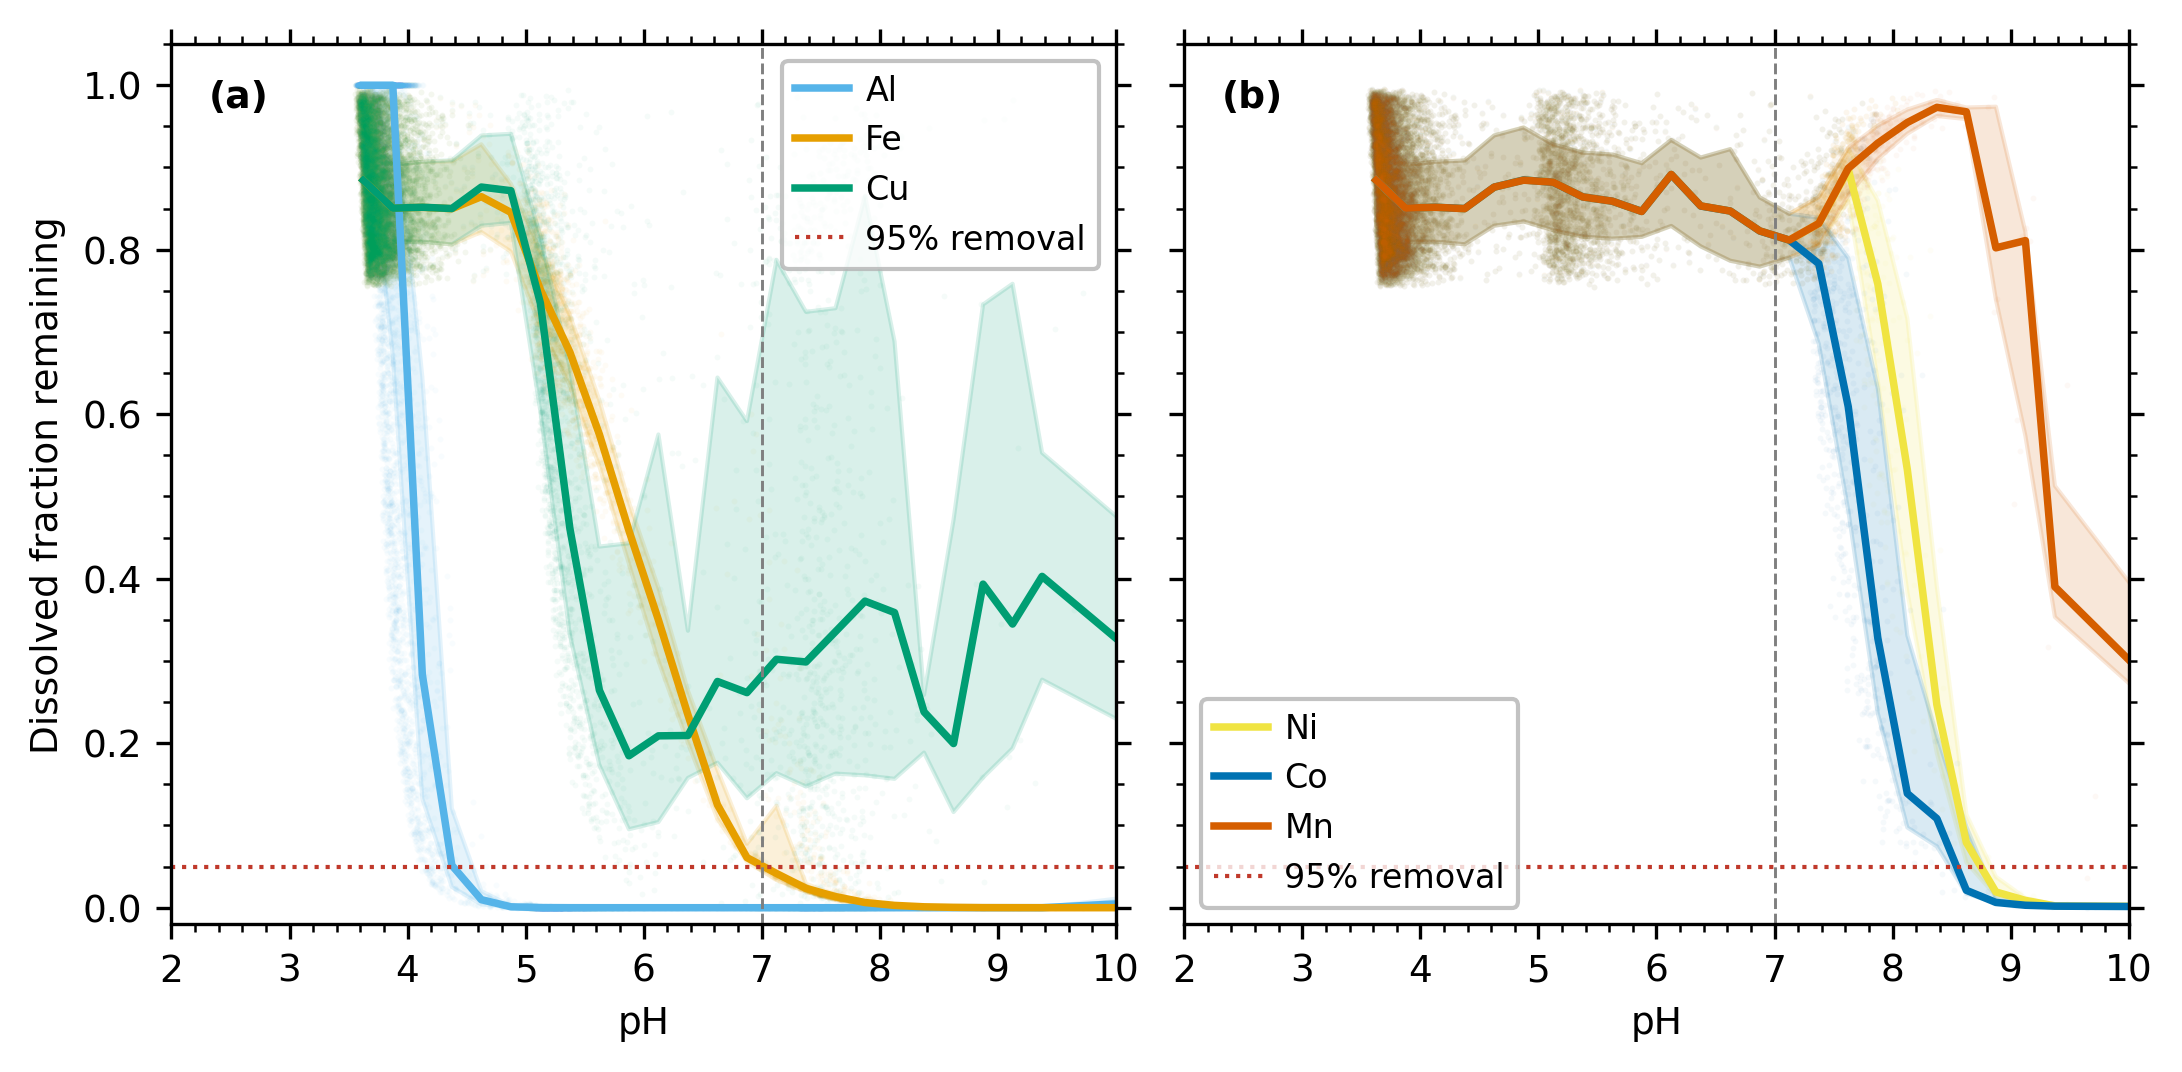
\includegraphics[width=0.95\linewidth]{results/Leach_recovery_UP6/figN2_recovery_curves_eq.png}
  \caption{\textbf{Dissolved metal fraction remaining as a function of pH under phase-equilibrium conditions.}
  Results span 12{,}001 sampled leachate compositions.
  \textbf{(a)} Early-precipitating metals (Al, Fe, Cu): Al and Fe undergo sharp, composition-insensitive transitions below pH~5; Cu exhibits a two-stage profile, a plateau driven by sulfate-complex buffering followed by an abrupt transition once the complex dissociates.
  \textbf{(b)} Late-precipitating metals (Ni, Co, Mn): Ni and Co removal curves overlap within $\Delta$pH~$\leq$~0.3 across all compositions, confirming that their fractionation by pH control alone is thermodynamically impossible; Mn remains largely dissolved through pH~9.
  Solid lines: median; shaded bands: interquartile range (IQR); faint scatter: individual simulations; dashed segments: sparsely sampled pH bins. (Best viewed in color; refer to the online version for interpretation.)}
    \label{fig:recovery}
\end{figure}

%%%%%%%
%%%%%%% Figure~\ref{fig:recovery}
%%%%%%% Figure~\ref{fig:recovery}
%%%%%%%

% Removal curves translate thermodynamic onset into process metrics.
Figure~\ref{fig:recovery} translates the thermodynamic precipitation sequence into directly measurable, process-relevant quantities: the dissolved fraction remaining for each metal as a function of pH. The layout separates the early-precipitating metals (Al, Fe, Cu) from the late group (Ni, Co, Mn), making the contrast in removal behavior. Fe and Al removal transitions are sharp and composition-insensitive, consistent with their large thermodynamic driving forces and the absence of competing speciation pathways that would introduce compositional sensitivity~\cite{stumm_aquatic_1996, may_gibbsite_1979}. Al's transition is centered $\sim$0.5 pH units lower than Fe, reflecting the lower $K_{sp}$ of Al(OH)$_3$(s); the somewhat broader interquartile range (IQR) of the Al transition reflects compositional variability in Al loading and ionic strength across the leachate ensemble, rather than competing speciation pathways.

Cu presented a delayed-onset, compositionally sensitive removal profile distinct from Al and Fe. The median dissolved fraction remained near 85--90\% through pH~$\approx$~4.5, then fell steeply to $\sim$20--25\% by pH~6 as free Cu$^{2+}$ activity crossed the $K_{sp}(\text{Cu(OH)}_2)/[\text{OH}^-]^2$ threshold once the CuSO$_4$ complex dissociated~\cite{crundwell_extractive_2011, stumm_aquatic_1996}. Unlike Al and Fe, Cu did not approach quantitative removal within the studied pH range; instead, the median plateaued at $\sim$20--25\% with a substantially wider interquartile range (IQR), reflecting strong sensitivity of the removal efficiency to leachate composition~\cite{virolainen_removal_2017}. A model that ignores sulfate complexation and equates total dissolved Cu with free Cu$^{2+}$ activity would predict an earlier, steeper removal onset resembling the Al and Fe profiles, and would fail to reproduce the delayed onset and the elevated residual dissolved fraction observed here. The apparent rise in the Cu median above pH~8 in Fig.~\ref{fig:recovery}(a) is a sparse-data artifact: the separate-beakers analogue delivers very few simulated compositions to this pH range, and the interpolated dashed segments carry no physical significance.

The most process-critical feature of the late-precipitating group (Fig.~\ref{fig:recovery}(b)) is the near-complete overlap of the Ni and Co removal curves. Both metals begin meaningful removal above pH~7--8 and their median dissolved fractions, IQR bands, and removal trajectories track one another within a window of $\leq$0.3 pH units across the full 12{,}001-sample ensemble. This near-degeneracy is a direct thermodynamic consequence of the proximity of their hydroxide solubility products: $\log K_{sp}({\rm Co(OH)_2}) \approx -15.6$ and $\log K_{sp}({\rm Ni(OH)_2}) \approx -15.3$~\cite{noauthor_ksp_nodate, bard_electrochemical_2022}, a difference of less than 0.3 log units that translates directly into the sub-0.3-pH-unit separation window observed here. The Co(OH)$_2$(s)--Ni(OH)$_2$(s) selectivity window of $\Delta$pH~$\approx$~0.3 is too narrow to support reliable fractionation by pH control alone in a single-stage hydroxide process~\cite{free_hydrometallurgy_2021, zanoletti_review_2024, larouche_progress_2020}. This fundamental limitation is well-established in battery hydrometallurgy: industrial flowsheets universally resort to solvent extraction using acidic organophosphorus extractants that coordinate through the phosphoryl oxygen (P=O), such as Cyanex~272 (phosphinic acid), D2EHPA (phosphoric acid ester), or PC88A (phosphonic acid monoester), to achieve the Co/Ni separation that precipitation thermodynamics cannot deliver~\cite{rickelton_cobalt-nickel_1984, preston_solvent_1982, swain_separation_2015, swain_separation_2016, virolainen_removal_2017, rabah_recovery_2008}. Their selectivity for Co$^{2+}$ over Ni$^{2+}$ arises from the substantially larger stability of Co$^{2+}$--phosphoryl complexes, providing a thermodynamic driving force for separation that the $\Delta\log K_{sp} \approx 0.3$ between Co(OH)$_2$(s) and Ni(OH)$_2$(s) cannot offer~\cite{rickelton_cobalt-nickel_1984, preston_solvent_1982}. The narrow IQR bands of both Ni and Co confirm that this co-precipitation behavior is composition-insensitive, a thermodynamic feature independent of cathode chemistry. Mn removal onset occurred near pH~8, approximately 0.5--1 pH units above Ni and Co~\cite{free_hydrometallurgy_2021, larouche_progress_2020}.

\begin{figure}[!h]
  \centering
  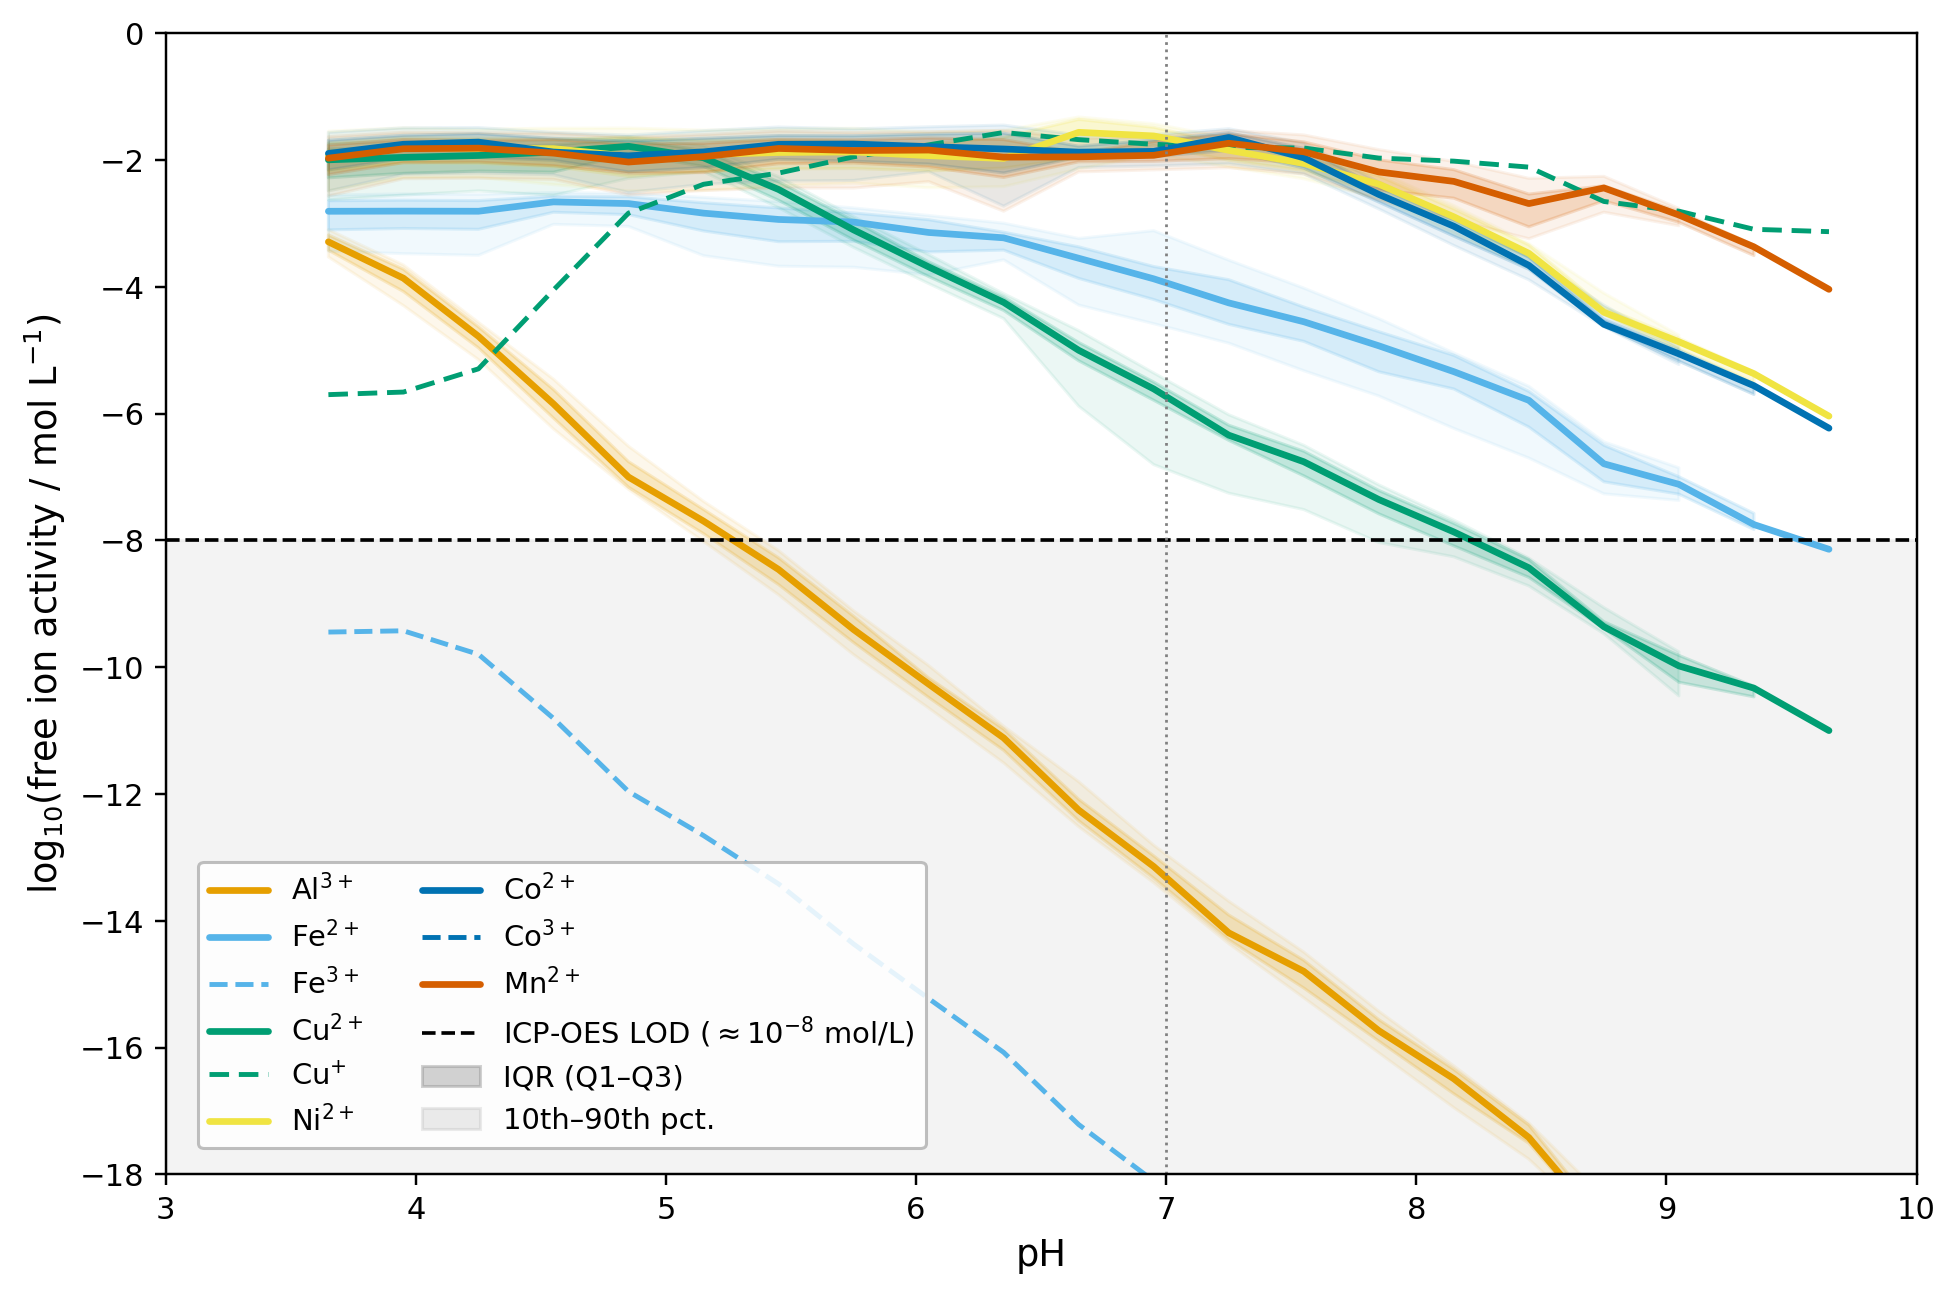
\includegraphics[width=\linewidth]{results/Leach_recovery_UP6/figN3_free_ion_activity_eq.png}
  \caption{\textbf{Free-ion activity suppression as a function of pH under phase-equilibrium conditions.}
  Median log$_{10}$(free-ion activity) for the dominant aqueous species of each metal across 12{,}001 sampled leachate compositions. For Fe, both Fe$^{2+}$ (solid) and Fe$^{3+}$ (dashed) are shown; at pe~$\approx$~6.35, Fe$^{3+}$ is redox-suppressed relative to Fe$^{2+}$ and lies below the LOD throughout. For Co, Co$^{2+}$ (solid) and Co$^{3+}$ (dashed) are shown; Co$^{3+}$ is similarly suppressed below the LOD. Shaded bands: dark inner band, interquartile range (Q1--Q3); light outer band, 10th--90th percentile range; drawn for the primary oxidation state only. Horizontal dashed line: ICP-OES limit of detection (LOD, $\approx 10^{-8}$\,mol/L); gray zone below this line is analytically inaccessible. Vertical dotted line: pH~7.}
  \label{fig:free_ion}
\end{figure}

%%%%%%
%%%%%%
%%%%%%

Understanding where ICP-OES feedback remains a reliable proxy for precipitation driving force and where it does not is essential for designing closed-loop SDL dosing protocols. Figure~\ref{fig:free_ion} shows that as pH increased, the free-ion activity of each metal declined steeply, in most cases falling below the ICP-OES limit of detection (LOD, $\approx 10^{-8}$\,mol/L) well before total dissolved metal was exhausted. Because ICP-OES measures total dissolved metal rather than free-ion activity, these two quantities diverged progressively as speciation shifted toward complexed forms. This divergence defined a practical \emph{analytical horizon}: the pH above which the thermodynamically active free-ion fraction became analytically invisible even while measurable dissolved metal persisted~\cite{stumm_aquatic_1996}. For SDL systems relying on ICP-OES as the sole feedback channel, the ICP-OES signal progressively decouples from the free-ion activity driving precipitation as pH increases, eventually reaching this horizon beyond which the thermodynamically active fraction is undetectable even while total dissolved metal persists; supplementary analytical channels sensitive to speciated rather than total dissolved metal are therefore required to maintain reliable closed-loop pH control above this threshold.

Iron presented the most important redox complication. Although Fe(OH)$_3$(s) precipitation is governed by Fe$^{3+}$ activity, the simulated redox state (pe~$\approx$~6.35) suppressed Fe$^{3+}$ by nearly seven orders of magnitude relative to Fe$^{2+}$, placing a$_{\rm Fe^{3+}}$ below the LOD throughout the entire pH range. The analytically accessible dissolved Fe pool is therefore Fe$^{2+}$, which crossed the LOD near pH~7 as Fe(OH)$_3$(s) removed dissolved Fe from solution. Consequently, ICP-OES total-Fe measurements track dissolved Fe$^{2+}$ rather than the free Fe$^{3+}$ fraction that drives precipitation onset~\cite{stumm_aquatic_1996}.

Al$^{3+}$ activity crossed the LOD near pH~5.2 and fell to analytically undetectable levels by pH~5.5, as Al(OH)$_3$(s) precipitation pinned the free-ion activity. Cu$^{2+}$, Ni$^{2+}$, Co$^{2+}$, and Mn$^{2+}$ free-ion activities clustered near $10^{-2}$\,mol/L at acidic pH and remained above the LOD through neutral pH. For Cu, the free Cu$^{2+}$ activity was pinned by $K_{sp}(\text{Cu(OH)}_2)$ above pH~5, while total dissolved Cu declined more slowly owing to the CuSO$_4$ complex reservoir; equating ICP-OES total-Cu measurements with free-ion activity above this pH systematically overestimates the thermodynamic driving force for further precipitation~\cite{crundwell_extractive_2011, stumm_aquatic_1996}. Co$^{3+}$, shown as a dashed line alongside Co$^{2+}$, remained below the LOD throughout, mirroring the Fe$^{3+}$ suppression; at pe~$\approx$~6.35 the Nernst equilibrium strongly favors Co$^{2+}$, and Co$^{3+}$ played no role in dissolved Co speciation or Co(OH)$_2$(s) precipitation kinetics.

Taken together, Figs.~\ref{fig:speciation_panel}--\ref{fig:free_ion} reveal three interconnected layers governing the selectivity of pH-staged neutralization: the thermodynamic precipitation sequence set by relative $K_{sp}$ values; the speciation-dependent partitioning of dissolved metal between free and complexed forms, which shifts effective precipitation onset pH; and the analytical visibility window of each metal, which constrains what ICP-OES can resolve and where feedback control remains reliable. These layers define the operating envelope of model-guided selective precipitation and provide quantitative design criteria for autonomous neutralization protocols in self-driving laboratory systems.

%%%%%%
%%%%%%
%%%%%%

\subsection{High-Throughput Experimental Mapping of Leaching/Recovery Processes}

Figure~\ref{fig:ICP_exp} presents the experimental validation of the thermodynamic precipitation sequence using a HTE SDL platform. A factorial matrix spanning five leachate dilution levels (5--50\% v/v) and ten NaOH addition levels (0--1.0 equivalents) was executed on a fixed NMC532 battery leachate, providing 50 conditions per metal with full ICP-OES quantification at each condition (Fig.~\ref{fig:ICP_exp}(a)).

\begin{figure*}[!h]
    \centering
    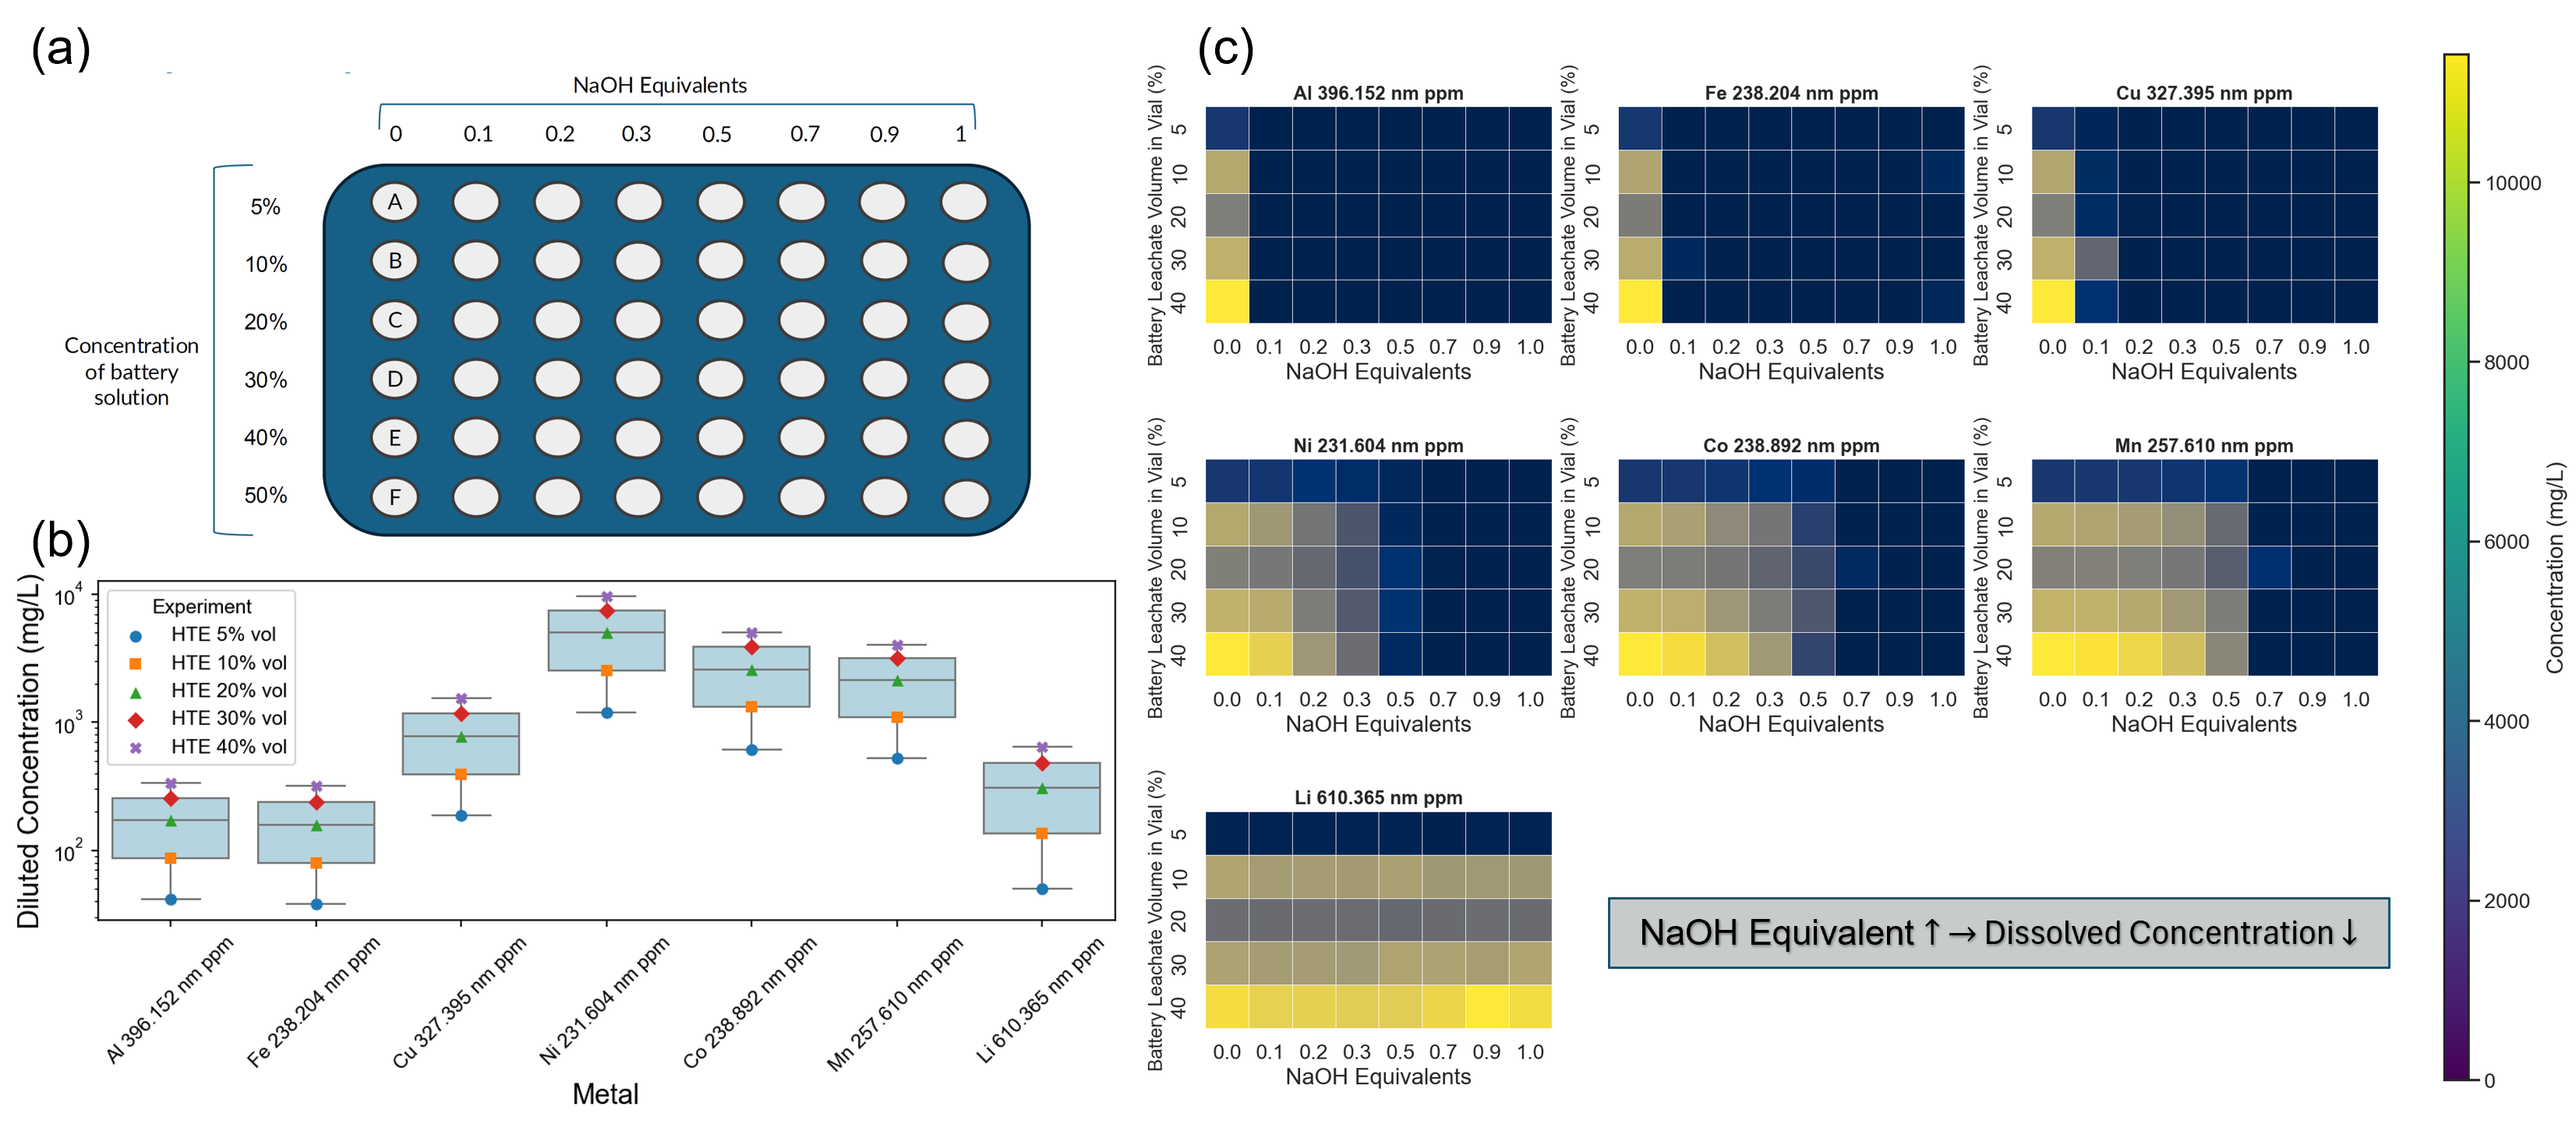
\includegraphics[width=0.95\linewidth]{ICP/Figure_Experimental_Results_Paper.png}
    \caption{\textbf{High-throughput ICP-OES mapping of NMC532 leachate neutralization across a factorial dilution--alkalinity matrix.}
    (a) Schematic of the SDL experimental design: six leachate dilution levels crossed with eight NaOH addition levels (0--1.0 equivalents) on a fixed NMC532 battery leachate.
    (b) Baseline dissolved metal concentrations (mg\,L$^{-1}$, log scale) at NaOH = 0 across all dilution conditions; individual symbols denote dilution level. Ni dominates the dissolved inventory, consistent with NMC532 stoichiometry; the spread within each metal reflects the dilution range.
    (c) Process maps showing ICP-OES dissolved concentration (color scale, mg\,L$^{-1}$) as a function of NaOH equivalents ($x$-axis) and leachate dilution ($y$-axis) for each metal. Al and Fe are removed at the lowest NaOH doses; Cu at intermediate doses; Ni and Co co-precipitate at higher doses; Mn persists across the full range; Li is unaffected at all conditions.}
    \label{fig:ICP_exp}
\end{figure*}

The baseline characterization at NaOH = 0 (Fig.~\ref{fig:ICP_exp}(b)) confirmed that Ni dominated the dissolved metal inventory at all dilution levels, consistent with the high Ni stoichiometry of NMC532 cathode material. Co and Mn followed at comparable concentrations, then Cu, with Al and Fe present at the lowest levels. The spread within each metal across the six dilution conditions reflected the expected linear scaling of dissolved concentration with leachate fraction. This baseline distribution is in qualitative agreement with the model input compositions (Table~\ref{tab:baseline_leachate}), establishing a shared chemical anchor between the thermodynamic calculations and the experimental measurements.

The thermodynamic model and the SDL platform were designed to work in a complementary fashion. The predicted precipitation sequence, onset pH values, and selectivity windows informed the choice of experimental conditions: the NaOH equivalent range (0--1.0) was intended to span the full predicted precipitation cascade from Al(OH)$_3$(s) through Mn(OH)$_2$(s), and the dilution range was chosen to probe the concentration dependence of onset behavior suggested by the uncertainty analysis. 
The factorial matrix of 48 conditions (6 dilution levels $\times$ 8 NaOH equivalents) was executed in a single automated SDL run, with each condition analyzed by ICP-OES to yield simultaneous concentrations of all seven metals, yielding 48 analyses covering the full dilution--alkalinity space in one unattended run. The process maps (Fig.~\ref{fig:ICP_exp}(c)) revealed a precipitation ordering that closely matched the thermodynamic sequence predicted by the model. Al and Fe were removed at the lowest NaOH equivalents ($\lesssim$0.1), transitioning abruptly to near-zero dissolved concentration independent of dilution level, consistent with their low $K_{sp}$ values and large thermodynamic driving forces. Cu removal followed at intermediate NaOH equivalents (0.1--0.3), with the transition showing moderate dilution dependence, qualitatively consistent with the sulfate-complex buffering mechanism identified in the speciation analysis. Ni and Co process maps were strikingly similar: both metals persisted in solution through intermediate NaOH additions and transitioned to low dissolved concentrations over the same narrow range of equivalents, providing direct experimental confirmation of their thermodynamic near-degeneracy. Mn was the most recalcitrant: it remained at elevated dissolved concentrations even at 1.0 NaOH equivalents, particularly at lower dilution levels, confirming that quantitative Mn removal requires alkalinity beyond the range investigated here, consistent with the model prediction of a median onset pH~$\approx$~12.6. Li maintained high dissolved concentrations across all NaOH doses and dilution levels, confirming its thermodynamic inertness toward hydroxide precipitation under these conditions.

The dilution axis in Fig.~\ref{fig:ICP_exp}(c) provides a complementary perspective on how absolute metal loading modulates the NaOH demand. At higher leachate fractions (lower dilution), the absolute metal concentrations are greater, shifting the effective precipitation threshold to higher NaOH equivalents for the later-precipitating metals (Ni, Co, Mn). This dilution dependence is thermodynamically expected: the saturation condition $Q_p = K_{sp}^p$ must be reached through the combined effect of pH increase and the absolute free-ion activity, both of which are functions of dilution. Al and Fe, by contrast, showed negligible dilution dependence, consistent with their large thermodynamic driving forces overwhelming any activity-level effects within this dilution range.

Bridging the quantitative gap between model and experiment is the natural next step: using the thermodynamic model's predicted uncertainty in onset pH and selectivity windows to select maximally informative experimental conditions via Bayesian optimization would close the loop between simulation and SDL, enabling autonomous convergence on optimal NaOH dosing strategies for any target leachate composition.



%%%%%
%%%%%
%%%%%

\section{Conclusions}\label{sec:conclusions}

Thermodynamic modeling of NaOH neutralization across 12{,}001 simulated leachate compositions, spanning NMC, NCA, and LCO cathode chemistries, established that hydroxide precipitation in multicomponent battery leachates follows a robust, thermodynamically ordered sequence: Al(OH)$_3$(s) $\to$ Fe(OH)$_3$(s) $\to$ Cu(OH)$_2$(s) $\to$ Co(OH)$_2$(s) $\approx$ Ni(OH)$_2$(s) $\to$ Mn(OH)$_2$(s). This hierarchy was conserved across the full compositional space, confirming that it reflects the relative solubility products of these phases within the concentration ranges characteristic of battery leachates rather than being composition-specific.

Rigorous activity modeling using the Specific Ion Interaction Theory (SIT) proved essential. At ionic strengths of $\sim$2~mol~kg$^{-1}$, sulfate complexation sequestered a substantial fraction of dissolved Ni$^{2+}$, Cu$^{2+}$, and Mn$^{2+}$ as neutral ion pairs, reducing free-ion activities well below total dissolved concentrations and shifting precipitation onset to higher pH than simpler models predict. Models that equate total dissolved metal with free-ion activity systematically overestimate the thermodynamic driving force for precipitation, producing onset pH predictions that are too low.

The most process-critical finding was the near-degeneracy of Co(OH)$_2$(s) and Ni(OH)$_2$(s): their separation window of $\Delta$pH~$\approx$~0.3, a direct consequence of their nearly identical solubility products ($\Delta\log K_{sp} \approx 0.3$), renders their fractionation by pH control alone thermodynamically impossible. By contrast, the Cu(OH)$_2$(s)$\to$Co(OH)$_2$(s) gap of $\Delta$pH~$\approx$~2.2 defines a robust, exploitable window for selective removal of impurity metals (Al, Fe, Cu) before the valuable cathode metals begin to precipitate. These quantitative selectivity windows provide direct NaOH dose targets for model-guided process design.

High-throughput SDL experimentation across a factorial dilution--alkalinity matrix confirmed the qualitative precipitation ordering and the near-degeneracy of Ni and Co over 48 automated conditions, providing experimental grounding for the thermodynamic predictions. The divergence between free-ion activity and total dissolved concentration as pH increased further defined an analytical horizon beyond which ICP-OES feedback loses sensitivity to the thermodynamically active free-ion fraction, a constraint that must be accounted for in autonomous pH control strategies.

These results establish a quantitative thermodynamic foundation for selective metal recovery from battery leachates and delineate the physicochemical boundaries within which pH-staged neutralization can and cannot achieve fractionation. Three directions emerge naturally from this foundation. First, the Co/Ni near-degeneracy identified here defines a hard thermodynamic ceiling for hydroxide-only separation; overcoming it will require modifier strategies, including ionic-strength adjustment to shift relative activity coefficients, temperature excursions to exploit the differential enthalpy of dissolution ($\Delta H_{sp}$) of Co(OH)$_2$(s) vs.\ Ni(OH)$_2$(s), or the introduction of selective organic ligands such as the phosphinic (Cyanex~272) and phosphonic (PC88A) acid extractants that show markedly larger Co$^{2+}$/Ni$^{2+}$ separation factors than hydroxide. Second, bridging the remaining quantitative gap between thermodynamic prediction and experimental outcome calls for a multi-fidelity SDL campaign in which cheap, high-throughput thermodynamic simulations screen the modifier--pH--dilution space and nominate a sparse set of high-information experimental conditions for SDL validation, iterating until model and experiment converge. Third, the analytical horizon identified here, the pH above which free-ion activity falls below the ICP-OES detection limit while total dissolved metal persists, motivates the integration of ion-selective electrodes or in-line speciation probes as complementary feedback channels for closed-loop pH control. Pursuing these directions within a unified model-guided SDL framework represents the most direct path toward fully autonomous, composition-adaptive process design for battery recycling.

%%%%%%%%%%
%%%%%%%%%%
%%%%%%%%%%
%%%%%%%%%%

\section*{Declaration of Competing Interest}
The authors declare that they have no known competing financial interests or personal relationships that could have appeared to influence the work reported in this paper.

\section*{Acknowledgments}
\textcolor{red}{The authors acknowledge the support of Natural Resources Canada (NRCan) and the contributions of all project partners.}

\section*{Authors' Contributions}
\noindent
\textbf{V. Attari:} Conceptualization, thermodynamic modeling, writing (original draft), editing. \\
\textbf{C. Cronin:} High-throughput experimentation, data acquisition, writing (review and editing). \\
\textbf{B. Cao:} High-throughput experimentation, ICP analysis, writing (review and editing). \\
\textbf{R.\,P. Jansonius:} Experimental design \\
\textbf{M. Greenwood:} writing (review and editing). \\
\textbf{J. Hattrick-Simpers:} Funding acquisition, supervision, writing (review and editing).


\section*{Data Availability}
The thermodynamic modeling results, high-throughput experimental datasets, and ICP measurements reported in this study are available at GitHub Link (\url{}) or from the corresponding author upon reasonable request.

\section*{Appendix}


\subsection{Metal Hydroxide Solubility Constants}



For equilibrium modeling, the thermodynamic solubility product is recast into an equivalent formation reaction expressed in terms of fundamental aqueous components (metal cations, protons, and water),
\begin{equation}
\mathrm{M(OH)_n(s) = M^{n+} - nH^+ + nH_2O},
\end{equation}
which is thermodynamically equivalent to the precipitation reaction
\begin{equation}
\mathrm{M^{n+} + nH_2O \rightleftharpoons M(OH)_n(s) + nH^+}.
\end{equation}

Using the auto-ionization equilibrium of water, $\mathrm{H_2O \rightleftharpoons H^+ + OH^-}$ with equilibrium constant $K_w$, the corresponding formation constant is given by
\begin{equation}
K_{\mathrm{form}} = \frac{K_w^{\,n}}{K_{sp}},
\end{equation}
or, in logarithmic form,
\begin{equation}
\log K_{\mathrm{form}} = n \log K_w - \log K_{sp}.
\end{equation}

For example, for $\mathrm{Co(OH)_2(s)}$ with $K_{sp}=2.5\times10^{-16}$ ($\log K_{sp}=-15.60$), the resulting formation constant is $\log K_{\mathrm{form}}=12.40$, consistent with values reported in standard thermodynamic databases. These constants for a series of example metal hydroxide phases are summarized in Table~\ref{tab:ksp_hydroxides_updated}. While $K_{sp}$ (and thus $\Delta G^\circ$) fully determines precipitation selectivity at fixed temperature, the standard enthalpy change $\Delta H^\circ$ governs only the temperature dependence of equilibrium constants via the van~’t~Hoff relation. Consequently, $\Delta H^\circ$ does not influence precipitation order under isothermal conditions, but becomes relevant during aging, thermal excursions, or phase transformations, where slow re-equilibration can favor more thermodynamically stable polymorphs over metastable hydroxide phases.

%%%%%
%%%%%
%%%%%

\renewcommand{\thetable}{A\arabic{table}}
\setcounter{table}{0}

\begin{table*}[!ht]
\centering
\scriptsize
\caption{Thermodynamic constants for metal hydroxide phases at 25$^\circ$C.
Reactions are written in the formation (component-reaction) convention.}
\label{tab:ksp_hydroxides_updated}
\begin{tabular}{l l p{5.0cm} c c c c}
\hline
\textbf{Order} & \textbf{Phase} 
& \textbf{Reaction} 
& $\boldsymbol{K_{sp}}$ 
& $\boldsymbol{\log K_{sp}}$ 
& $\boldsymbol{\log K_w}$ 
& $\boldsymbol{\log K_{\text{form}}}$ \\
\hline
1 & Fe(OH)$_3$(cr) 
& Fe(OH)$_3$ = Fe$^{3+}$ -- 3H$^+$ + 3H$_2$O
& $10^{-38}$ & $-38.0$ & $-14$ & 1.22 \\

  & Fe(OH)$_3$(s) 
& Fe(OH)$_3$ = Fe$^{3+}$ -- 3H$^+$ + 3H$_2$O
& $10^{-38}$ & $-38.0$ & $-14$ & 2.78 \\

  & Fe(OH)$_3$(am) 
& Fe(OH)$_3$ = Fe$^{3+}$ -- 3H$^+$ + 3H$_2$O
& $10^{-38}$ & $-38.0$ & $-14$ & 3.50 \\

2 & Al(OH)$_3$(s) (Gibbsite)
& Al(OH)$_3$ = Al$^{3+}$ -- 3H$^+$ + 3H$_2$O
& $10^{-33}$ & $-33.0$ & $-14$ & 7.74 \\

3 & Cu(OH)$_2$(s) 
& Cu(OH)$_2$ = Cu$^{2+}$ -- 2H$^+$ + 2H$_2$O
& $1.6 \times 10^{-19}$ & $-19.6$ & $-14$ & 8.64 \\

4 & Ni(OH)$_2$(s) 
& Ni(OH)$_2$ = Ni$^{2+}$ -- 2H$^+$ + 2H$_2$O
& $5.0 \times 10^{-16}$ & $-15.3$ & $-14$ & 10.8 -- 11.0 \\

5 & Co(OH)$_2$(blue) 
& Co(OH)$_2$ = Co$^{2+}$ -- 2H$^+$ + 2H$_2$O
& $2.5 \times 10^{-16}$ & $-15.6$ & $-14$ & 12.2 \\

  & Co(OH)$_2$(rose--I) 
& Co(OH)$_2$ = Co$^{2+}$ -- 2H$^+$ + 2H$_2$O
& $2.5 \times 10^{-16}$ & $-15.6$ & $-14$ & 13.2 \\

  & Co(OH)$_2$(rose--II) 
& Co(OH)$_2$ = Co$^{2+}$ -- 2H$^+$ + 2H$_2$O
& $2.5 \times 10^{-16}$ & $-15.6$ & $-14$ & 13.8 \\

6 & Mn(OH)$_2$(s) 
& Mn(OH)$_2$ = Mn$^{2+}$ -- 2H$^+$ + 2H$_2$O
& $1.9 \times 10^{-13}$ & $-12.7$ & $-14$ & 15.3 \\
\hline
\end{tabular}
\end{table*}


%%%%%
%%%%%
%%%%%

\small
\bibliography{Hydrometallurgy,SDLs}
\bibliographystyle{elsarticle-num}
%\bibliographystyle{abbrv}

\end{document}
